\documentclass[11pt,a4paper,oneside]{report}             % Single-side
%\documentclass[11pt,a4paper,twoside,openright]{report}  % Duplex

\usepackage{ifxetex}
\ifxetex
  \usepackage{fontspec}
\else
  \usepackage[T1]{fontenc}
  \usepackage[utf8]{inputenc}
  \usepackage{lmodern}
\fi

\usepackage[magyar,english]{babel} % Alapértelmezés szerint utoljára definiált nyelv lesz aktív, de később külön beállítjuk az aktív nyelvet.

\usepackage{cmap}
\usepackage{amsfonts,amsmath,amssymb} % Mathematical symbols.
\usepackage[ruled,boxed,resetcount,linesnumbered]{algorithm2e} % For pseudocodes.
\usepackage{booktabs} % For publication quality tables for LaTeX
\usepackage{graphicx}

%\usepackage{fancyhdr}
%\usepackage{lastpage}

\usepackage{anysize}
\usepackage{sectsty}
\usepackage{setspace}  % Ettol a tablazatok, abrak, labjegyzetek maradnak 1-es sorkozzel!

\usepackage{hyperref} % For hyperlinks in the generated document. 
\usepackage{color}
\usepackage{listings} % For source code snippets.

\usepackage[amsmath,thmmarks]{ntheorem} % Theorem-like environments.

\usepackage[hang]{caption}
%\usepackage[final]{pdfpages}
%\usepackage[titletoc]{appendix}


%--------------------------------------------------------------------------------------
% Main variables

%TODO edit names and captions
%--------------------------------------------------------------------------------------
\newcommand{\vikszerzoVezeteknev}{Szepes}
\newcommand{\vikszerzoKeresztnev}{Nóra}
\newcommand{\vikkonzulensA}{Dr.~Sándor Gajdos} % Első konzulens neve
\newcommand{\vikkonzulensB}{Bence Golda} % Második konzulens neve; hagyd üresen, ha egy konzulensed van.
\newcommand{\vikcim}{Design and Implementation of an Educational Support System} % Cím
\newcommand{\viktanszek}{\bmetmit} % Tanszék
\newcommand{\vikdoktipus}{\bsc} % Dokumentum típusa (diplomaterv, szakdolgozat, TDK-dolgozat, stb.)
%
%%--------------------------------------------------------------------------------------
% TDK-specifikus változók
%--------------------------------------------------------------------------------------
\newcommand{\tdkszerzoB}{Második Szerző} % Második szerző neve; hagyd üresen, ha egyedül í­rtad a TDK-t.
\newcommand{\tdkev}{2014} % A dolgozat írásának éve (pl. "2014") (Ez OTDK-nál eltérhet az aktuális évtől.)

% További adatok az OTDK címlaphoz (BME-s TDK-hoz nem kell kitölteni)
\newcommand{\tdkevfolyamA}{IV} % Első szerző évfolyama, római számmal (pl. IV).
\newcommand{\tdkevfolyamB}{III} % Második szerző évfolyama, római számmal (pl. III).
\newcommand{\tdkkonzulensbeosztasA}{egyetemi tanár} % Első konzulens beosztása (pl. egyetemi docens)
\newcommand{\tdkkonzulensbeosztasB}{doktorandusz} % Második konzulens beosztása (pl. egyetemi docens)
\newcommand{\szerzoMeta}{\vikszerzoVezeteknev{} \vikszerzoKeresztnev} % egy szerző esetén
%\newcommand{\szerzoMeta}{\vikszerzoVezeteknev{} \vikszerzoKeresztnev, \tdkszerzoB} % két szerző esetén

\newcommand{\todo}[1]{\textcolor{red}{\textbf{***TODO***: #1}}}
\newcommand{\bence}[1]{\textcolor{green}{\textbf{*Bence*: #1}}}
\newcommand{\nori}[1]{\textcolor{blue}{\textbf{*Nóri*: #1}}}
\newcommand{\see}[1]{(see \refstruc{#1})}
\newcommand{\newparagraph}[1]{\paragraph{#1}\mbox{}\\}

%--------------------------------------------------------------------------------------
%TODO Language configuration -- choose one
%--------------------------------------------------------------------------------------
%%--------------------------------------------------------------------------------------
% Elnevezések
%--------------------------------------------------------------------------------------
\newcommand{\dolgozatnyelve}{\selectlanguage{magyar}}

\newcommand{\bme}{Budapesti Műszaki és Gazdaságtudományi Egyetem}
\newcommand{\vik}{Villamosmérnöki és Informatikai Kar}

\newcommand{\bmemit}{Méréstechnika és Információs Rendszerek Tanszék}

\newcommand{\keszitette}{Készítette}
\newcommand{\konzulens}{Konzulens}

\newcommand{\bsc}{Szakdolgozat}
\newcommand{\msc}{Diplomaterv}

\newcommand{\pelda}{Példa}
\newcommand{\definicio}{Definíció}
\newcommand{\tetel}{Tétel}

\newcommand{\bevezeto}{Bevezető}
\newcommand{\koszonetnyilvanitas}{Köszönetnyilvánítás}
\newcommand{\abrakjegyzeke}{Ábrák jegyzéke}
\newcommand{\tablazatokjegyzeke}{Táblázatok jegyzéke}
\newcommand{\irodalomjegyzek}{Irodalomjegyzék}
\newcommand{\fuggelek}{Függelék}

\newcommand{\szerzo}{\vikszerzoVezeteknev{} \vikszerzoKeresztnev}


\newcommand{\englishParagraph}{
	\setlength{\parindent}{0em} % angol nyelvű dokumentumokban jellemző
	\setlength{\parskip}{0.5em} % angol nyelvű dokumentumokban jellemző
	\nonfrenchspacing
}

\newcommand{\hungarianParagraph}{
	\setlength{\parindent}{2em} % angol nyelvű dokumentumokban jellemző
	\setlength{\parskip}{0em}   % angol nyelvű dokumentumokban jellemző
	\frenchspacing
}

\newcommand{\defaultParagraph}{
	\hungarianParagraph
}

\bibliographystyle{huplain}
  % Beállítások magyar nyelvű dolgozathoz
%--------------------------------------------------------------------------------------
% Elnevezések
%--------------------------------------------------------------------------------------
\newcommand{\dolgozatnyelve}{\selectlanguage{english}}

\newcommand{\bme}{Budapest University of Technology and Economics}
\newcommand{\vik}{Faculty of Electrical Engineering and Informatics}

\newcommand{\bmemit}{Department of Measurement and Information Systems}
\newcommand{\bmetmit}{Department of Telecommunications and Media Informatics}

\newcommand{\keszitette}{Candidate}
\newcommand{\konzulens}{Advisors}

\newcommand{\bsc}{Bachelor's Thesis}
\newcommand{\msc}{Master's Thesis}

\newcommand{\pelda}{Example}
\newcommand{\definicio}{Definition}
\newcommand{\tetel}{Theorem}

\newcommand{\bevezeto}{Introduction}
\newcommand{\koszonetnyilvanitas}{Acknowledgements}
\newcommand{\abrakjegyzeke}{List of Figures}
\newcommand{\tablazatokjegyzeke}{List of Tables}
\newcommand{\irodalomjegyzek}{Bibliography}
\newcommand{\fuggelek}{Appendix}

\newcommand{\szerzo}{\vikszerzoKeresztnev{} \vikszerzoVezeteknev}

\newcommand{\englishParagraph}{
	\setlength{\parindent}{0em} % angol nyelvű dokumentumokban jellemző
	\setlength{\parskip}{0.5em} % angol nyelvű dokumentumokban jellemző
	\nonfrenchspacing
}

\newcommand{\hungarianParagraph}{
	\setlength{\parindent}{2em} % angol nyelvű dokumentumokban jellemző
	\setlength{\parskip}{0em}   % angol nyelvű dokumentumokban jellemző
	\frenchspacing
}

\newcommand{\defaultParagraph}{
	\englishParagraph
}

\bibliographystyle{plain}
 % Settings for English documents


%--------------------------------------------------------------------------------------
% Page layout setup
%--------------------------------------------------------------------------------------
% we need to redefine the pagestyle plain
% another possibility is to use the body of this command without \fancypagestyle
% and use \pagestyle{fancy} but in that case the special pages
% (like the ToC, the References, and the Chapter pages)remain in plane style

\pagestyle{plain}
\marginsize{35mm}{25mm}{15mm}{15mm}

\setcounter{secnumdepth}{0}
\sectionfont{\large\upshape\bfseries}
\setcounter{secnumdepth}{2}

\sloppy % Margón túllógó sorok tiltása.
\widowpenalty=10000 \clubpenalty=10000 %A fattyú- és árvasorok elkerülése
\def\hyph{-\penalty0\hskip0pt\relax} % Kötőjeles szavak elválasztásának engedélyezése


%--------------------------------------------------------------------------------------
% Setup hyperref package
%--------------------------------------------------------------------------------------
\hypersetup{
    bookmarks=true,            % show bookmarks bar?
    unicode=false,              % non-Latin characters in Acrobat's bookmarks
    pdftitle={\vikcim},        % title
    pdfauthor={\szerzoMeta},    % author
    pdfsubject={\vikdoktipus}, % subject of the document
    pdfcreator={\szerzoMeta},   % creator of the document
    pdfproducer={},    % producer of the document
    pdfkeywords={},    % list of keywords (separate then by comma)
    pdfnewwindow=true,         % links in new window
    colorlinks=true,           % false: boxed links; true: colored links
    linkcolor=black,           % color of internal links
    citecolor=black,           % color of links to bibliography
    filecolor=black,           % color of file links
    urlcolor=black             % color of external links
}


%--------------------------------------------------------------------------------------
% Set up listings
%--------------------------------------------------------------------------------------
\definecolor{lightgray}{rgb}{0.95,0.95,0.95}
\lstset{
	basicstyle=\scriptsize\ttfamily, % print whole listing small
	keywordstyle=\color{black}\bfseries, % bold black keywords
	identifierstyle=, % nothing happens
	commentstyle=\color{green}, % green comments
	stringstyle=\scriptsize,
	showstringspaces=false, % no special string spaces
	aboveskip=3pt,
	belowskip=3pt,
	backgroundcolor=\color{lightgray},
	columns=flexible,
	keepspaces=true,
	escapeinside={(*@}{@*)},
	literate=*
		{á}{{\'a}}1	{é}{{\'e}}1	{í}{{\'i}}1	{ó}{{\'o}}1	{ö}{{\"o}}1	{ő}{{\H{o}}}1	{ú}{{\'u}}1	{ü}{{\"u}}1	{ű}{{\H{u}}}1
		{Á}{{\'A}}1	{É}{{\'E}}1	{Í}{{\'I}}1	{Ó}{{\'O}}1	{Ö}{{\"O}}1	{Ő}{{\H{O}}}1	{Ú}{{\'U}}1	{Ü}{{\"U}}1	{Ű}{{\H{U}}}1
} 	
\def\lstlistingname{lista}	


%--------------------------------------------------------------------------------------
% Set up theorem-like environments
%--------------------------------------------------------------------------------------
% Using ntheorem package -- see http://www.math.washington.edu/tex-archive/macros/latex/contrib/ntheorem/ntheorem.pdf

\theoremstyle{plain}
\theoremseparator{.}
\newtheorem{example}{\pelda}

\theoremseparator{.}
%\theoremprework{\bigskip\hrule\medskip}
%\theorempostwork{\hrule\bigskip}
\theorembodyfont{\upshape}
\theoremsymbol{{\large \ensuremath{\centerdot}}}
\newtheorem{definition}{\definicio}

\theoremseparator{.}
%\theoremprework{\bigskip\hrule\medskip}
%\theorempostwork{\hrule\bigskip}
\newtheorem{theorem}{\tetel}


%--------------------------------------------------------------------------------------
% Some new commands and declarations
%--------------------------------------------------------------------------------------
\newcommand{\code}[1]{{\upshape\ttfamily\scriptsize\indent #1}}
\newcommand{\doi}[1]{DOI: \href{http://dx.doi.org/\detokenize{#1}}{\raggedright{\texttt{\detokenize{#1}}}}} % A hivatkozások közt így könnyebb DOI-t megadni.

\DeclareMathOperator*{\argmax}{arg\,max}
%\DeclareMathOperator*[1]{\floor}{arg\,max}
\DeclareMathOperator{\sign}{sgn}
\DeclareMathOperator{\rot}{rot}


%--------------------------------------------------------------------------------------
% Setup captions
%--------------------------------------------------------------------------------------
\captionsetup[figure]{
	width=.75\textwidth,
	aboveskip=10pt}

\renewcommand{\captionlabelfont}{\bf}
%\renewcommand{\captionfont}{\footnotesize\it}


%--------------------------------------------------------------------------------------
% Redefine reference style
%--------------------------------------------------------------------------------------
\newcommand{\figref}[1]{\ref{fig:#1}.}
\renewcommand{\eqref}[1]{(\ref{eq:#1})}
\newcommand{\listref}[1]{\ref{listing:#1}.}
\newcommand{\sectref}[1]{\ref{sect:#1}}
\newcommand{\tabref}[1]{\ref{tab:#1}.}


%--------------------------------------------------------------------------------------
% Hyphenation exceptions
%--------------------------------------------------------------------------------------
\hyphenation{Shakes-peare Mar-seilles ár-víz-tű-rő tü-kör-fú-ró-gép}


\author{\vikszerzo}
\title{\viktitle}


%--------------------------------------------------------------------------------------
% Table of tsnts and the main text
%--------------------------------------------------------------------------------------
\begin{document}


%TODO These define uidelines -- remove these
%~~~~~~~~~~~~~~~~~~~~~~~~~~~~~~~~~~~~~~~~~~~~~~~~~~~~~~~~~~~~~~~~~~~~~~~~~~~~~~~~~~~~~~
%\pagenumbering{gobble}
\dolgozatnyelve
\hungarianParagraph
\singlespacing
%--------------------------------------------------------------------------------------
% Rovid formai es tartalmi tajekoztato
%--------------------------------------------------------------------------------------

\footnotesize
\begin{center}
\large
\textbf{\Large Általános információk, a diplomaterv szerkezete}\\
\end{center}

A diplomaterv szerkezete a BME Villamosmérnöki és Informatikai Karán:
\begin{enumerate}
\item	Diplomaterv feladatkiírás
\item	Címoldal
\item	Tartalomjegyzék
\item	A diplomatervező nyilatkozata az önálló munkáról és az elektronikus adatok kezeléséről
\item	Tartalmi összefoglaló magyarul és angolul
\item	Bevezetés: a feladat értelmezése, a tervezés célja, a feladat indokoltsága, a diplomaterv felépítésének rövid összefoglalása
\item	A feladatkiírás pontosítása és részletes elemzése
\item	Előzmények (irodalomkutatás, hasonló alkotások), az ezekből levonható következtetések
\item	A tervezés részletes leírása, a döntési lehetőségek értékelése és a választott megoldások indoklása
\item	A megtervezett műszaki alkotás értékelése, kritikai elemzése, továbbfejlesztési lehetőségek
\item	Esetleges köszönetnyilvánítások
\item	Részletes és pontos irodalomjegyzék
\item	Függelék(ek)
\end{enumerate}

Felhasználható a következő oldaltól kezdődő \LaTeX diplomatervsablon dokumentum tartalma. 

A diplomaterv szabványos méretű A4-es lapokra kerüljön. Az oldalak tükörmargóval készüljenek (mindenhol 2,5~cm, baloldalon 1~cm-es kötéssel). Az alapértelmezett betűkészlet a 12 pontos Times New Roman, másfeles sorközzel, de ettől kismértékben el lehet térni, ill. más betűtípus használata is megengedett.

Minden oldalon -- az első négy szerkezeti elem kivételével -- szerepelnie kell az oldalszámnak.

A fejezeteket decimális beosztással kell ellátni. Az ábrákat a megfelelő helyre be kell illeszteni, fejezetenként decimális számmal és kifejező címmel kell ellátni. A fejezeteket decimális aláosztással számozzuk, maximálisan 3 aláosztás mélységben (pl. 2.3.4.1.). Az ábrákat, táblázatokat és képleteket célszerű fejezetenként külön számozni (pl. 2.4. ábra, 4.2 táblázat vagy képletnél (3.2)). A fejezetcímeket igazítsuk balra, a normál szövegnél viszont használjunk sorkiegyenlítést. Az ábrákat, táblázatokat és a hozzájuk tartozó címet igazítsuk középre. A cím a jelölt rész alatt helyezkedjen el.

A képeket lehetőleg rajzoló programmal készítsék el, az egyenleteket egyenlet-szerkesztő segítségével írják le (A \LaTeX~ehhez kézenfekvő megoldásokat nyújt).

Az irodalomjegyzék szövegközi hivatkozása történhet a Harvard-rendszerben (a szerző és az évszám megadásával) vagy sorszámozva. A teljes lista névsor szerinti sorrendben a szöveg végén szerepeljen (sorszámozott irodalmi hivatkozások esetén hivatkozási sorrendben). A szakirodalmi források címeit azonban mindig az eredeti nyelven kell megadni, esetleg zárójelben a fordítással. A listában szereplő valamennyi publikációra hivatkozni kell a szövegben (a \LaTeX-sablon a Bib\TeX~segítségével mindezt automatikusan kezeli). Minden publikáció a szerzők után a következő adatok szerepelnek: folyóirat cikkeknél a pontos cím, a folyóirat címe, évfolyam, szám, oldalszám tól-ig. A folyóiratok címét csak akkor rövidítsük, ha azok nagyon közismertek vagy nagyon hosszúak. Internetes hivatkozások megadásakor fontos, hogy az elérési út előtt megadjuk az oldal tulajdonosát és tartalmát (mivel a link egy idő után akár elérhetetlenné is válhat), valamint az elérés időpontját.

\vspace{5mm}
Fontos:
\begin{itemize}
	\item A szakdolgozatkészítő / diplomatervező nyilatkozata (a jelen sablonban szereplő szövegtartalommal) kötelező előírás, Karunkon ennek hiányában a szakdolgozat/diplomaterv nem bírálható és nem védhető!
	\item Mind a dolgozat, mind a melléklet maximálisan 15~MB méretű lehet!
\end{itemize}

\vspace{5mm}
\begin{center}
Jó munkát, sikeres szakdolgozatkészítést, ill. diplomatervezést kívánunk!
\end{center}

\normalsize
\onehalfspacing
\defaultParagraph

%%--------------------------------------------------------------------------------------
% Feladatkiiras (a tanszeken atveheto, kinyomtatott valtozat)
%--------------------------------------------------------------------------------------
\clearpage
\begin{center}
\large
\textbf{FELADATKIÍRÁS}\\
\end{center}

A feladatkiírást a tanszéki adminisztrációban lehet átvenni, és a leadott munkába eredeti, tanszéki pecséttel ellátott és a tanszékvezető által aláírt lapot kell belefűzni (ezen oldal \emph{helyett}, ez az oldal csak útmutatás). Az elektronikusan feltöltött dolgozatban már nem kell beleszerkeszteni ezt a feladatkiírást.



%TODO Titlepage -- choose one from below
%~~~~~~~~~~~~~~~~~~~~~~~~~~~~~~~~~~~~~~~~~~~~~~~~~~~~~~~~~~~~~~~~~~~~~~~~~~~~~~~~~~~~~~
	%--------------------------------------------------------------------------------------
%	The title page
%--------------------------------------------------------------------------------------
\begin{titlepage}
\begin{center}

\includegraphics[width=60mm,keepaspectratio]{figures/bme_logo.pdf}\\
\vspace{0.3cm}
\textbf{\bme}\\
\textmd{\vik}\\
\textmd{\viktanszek}\\[5cm]

\vspace{0.4cm}
{\huge \bfseries \vikcim}\\[0.8cm]
\vspace{0.5cm}
\textsc{\Large \vikdoktipus}\\[4cm]

{
	\renewcommand{\arraystretch}{0.85}
	\begin{tabular}{cc}
	 \makebox[7cm]{\emph{\keszitette}} & \makebox[7cm]{\emph{\konzulens}} \\ \noalign{\smallskip}
	 \makebox[7cm]{\szerzo} & \makebox[7cm]{\vikkonzulensA} \\
	  & \makebox[7cm]{\vikkonzulensB} \\
	\end{tabular}
}

\vfill
{\large 2015}
\end{center}
\end{titlepage}


		   % Szakdolgozat/Diplomaterv címlap
	%%% TDK címlap
\begin{titlepage}
  \begin{center}  
  
\includegraphics[width=7cm]{./figures/bme_logo.pdf}
  \vspace{0.3cm}
  
  \bme \\
  \vik \\
  \viktanszek \\
  \vspace{5cm}
  
  \huge {\vikcim}
  \vspace{1.5cm}
  
  \large {\textbf{\vikdoktipus}}
  \vfill
    
  {\Large 
  	\keszitette: \\ \vspace{0.3cm}
  	\szerzo \\
	\tdkszerzoB \\
  	\vspace{1.5cm}
  	\konzulens: \\ \vspace{0.3cm}
  	\vikkonzulensA \\
  	\vikkonzulensB \\
  }
  
  \vspace{2cm}
  \large {\tdkev.}
 \end{center}
\end{titlepage}
%% Címlap vége	% TDK címlap
	%%% OTDK külső címlap
\begin{titlepage}
  	$\;$ 
	\vspace{5cm}
	
	\begin{center}
	\Huge
	\textbf{TDK-dolgozat}\let\thefootnote\relax\footnote{A dolgozat bemutatását a XXXXXXXXX  ``Lorem ipsum dolor sit amet'' című program támogatta.}
	\end{center}
	
	\vspace{13cm}
	
	\Large
	\hspace{8cm} \szerzo
	
	\hspace{8cm} \tdkszerzoB
	
	\hspace{8cm} \tdkev.
\end{titlepage}

\newpage
\thispagestyle{empty}


%% OTDK belső címlap
\begin{titlepage}
  \begin{center}  
  
\includegraphics[width=7cm]{./figures/bme_logo.pdf}
  \vspace{0.3cm}
  
  \bme \\
  \vik \\
  \viktanszek \\
  \vspace{3.5cm}
  
  \huge {\vikcim}
  \vspace{1.5cm}
  
  \large {\textbf{\vikdoktipus}}
  \vfill
    
  {\Large 
  	{\large \keszitette:} \\ \vspace{0.2cm}
  	\szerzo \\ \tdkevfolyamA. évfolyam \\
	\vspace{0.5cm}
	\tdkszerzoB \\ \tdkevfolyamB. évfolyam \\
  	\vspace{1.5cm}
  	{\large \konzulens:} \\ \vspace{0.2cm}
  	\vikkonzulensA,\\ \tdkkonzulensbeosztasA \\
  	\vspace{0.5cm}
  	\vikkonzulensB,\\ \tdkkonzulensbeosztasB \\
  }
  
  \vspace{2cm}
  \large {\tdkev.}
  
 \end{center}
\end{titlepage}   % OTDK címlap
 

% Table of Contents
%~~~~~~~~~~~~~~~~~~~~~~~~~~~~~~~~~~~~~~~~~~~~~~~~~~~~~~~~~~~~~~~~~~~~~~~~~~~~~~~~~~~~~~
	\renewcommand{\contentsname}{Table of Contents}%
	\tableofcontents\vfill
	\thispagestyle{empty}
	\addtocontents{toc}{\protect\thispagestyle{empty}}


% Declaration and Abstract
%~~~~~~~~~~~~~~~~~~~~~~~~~~~~~~~~~~~~~~~~~~~~~~~~~~~~~~~~~~~~~~~~~~~~~~~~~~~~~~~~~~~~~~
%TODO your own content
	\selectlanguage{magyar}
\pagenumbering{gobble}
%--------------------------------------------------------------------------------------
% Nyilatkozat
%--------------------------------------------------------------------------------------
\begin{center}
\large
\textbf{HALLGATÓI NYILATKOZAT}\\
\end{center}

Alulírott \emph{\vikszerzoVezeteknev{} \vikszerzoKeresztnev}, szigorló hallgató kijelentem, hogy ezt a szakdolgozatot meg nem engedett segítség nélkül, saját magam készítettem, csak a megadott forrásokat (szakirodalom, eszközök stb.) használtam fel. Minden olyan részt, melyet szó szerint, vagy azonos értelemben, de átfogalmazva más forrásból átvettem, egyértelműen, a forrás megadásával megjelöltem.

Hozzájárulok, hogy a jelen munkám alapadatait (szerző(k), cím, angol és magyar nyelvű tartalmi kivonat, készítés éve, konzulens(ek) neve) a BME VIK nyilvánosan hozzáférhető elektronikus formában, a munka teljes szövegét pedig az egyetem belső hálózatán keresztül (vagy autentikált felhasználók számára) közzétegye. Kijelentem, hogy a benyújtott munka és annak elektronikus verziója megegyezik. Dékáni engedéllyel titkosított diplomatervek esetén a dolgozat szövege csak 3 év eltelte után válik hozzáférhetővé.

\begin{flushleft}
\vspace*{1cm}
Budapest, \today
\end{flushleft}

\begin{flushright}
 \vspace*{1cm}
 \makebox[7cm]{\rule{6cm}{.4pt}}\\
 \makebox[7cm]{\emph{\vikszerzoVezeteknev{} \vikszerzoKeresztnev}}\\
 \makebox[7cm]{hallgató}
\end{flushright}
\thispagestyle{empty}

\vfill
\clearpage
\thispagestyle{empty} % an empty page

\dolgozatnyelve %TODO Hallgatói nyilatkozat -- TDK és OTDK esetén törlendő!
	\pagenumbering{roman}
\setcounter{page}{1}

\selectlanguage{magyar}
\hungarianParagraph


%----------------------------------------------------------------------------
% Abstract in Hungarian
%----------------------------------------------------------------------------
\chapter*{Kivonat}\addcontentsline{toc}{chapter}{Kivonat}

A Szoftver Laboratórium 5 tantárgy lebonyolítása több száz hallgató adminisztratív feladatainak elvégzését is igényli az órák megtartása mellett. Ezen feladatok elvégzése egy adminisztrációs portál segítségével jelentősen megkönnyíthető. A tantárgy már eddig is rendelkezett egy portállal, de az évek során a tantárgy és a követelményrendszer változásával, illetve a felhasználók újabb elvárásai miatt elavultá vált. 

A szakdolgozatom célja egy új portál tervezése és a hozzátartozó vékony kliens implementálása, amely rugalmasan alkalmazkodik a követelményrendszer változásaihoz, illetve lehetőséget nyújt több tantárgy kezeléséhez is. A végleges rendszer három modult fog tartalmazni, mind a back end, mind a front end részen: a hallgatói, az oktatói és az admin modult. Ezen szakdolgozatban a hallgatói modul tervezése és elkészítése kerül bemutatásra.

A munkám során az előző portál specifikációját és az új elvárásokat vizsgálva elkészítettem az új rendszer specifikációját. A specifikálás során olyan technológiákkal ismerkedtem meg, mellyekkel előtérbe kerül a validáció és a verifikáció fontossága. Az így kapott specifikáció alapján megterveztem a kliens dizájnját ügyelve arra, hogy a minimalista, de egyszerűen kezelhető felhasználói felület csak a szükséges információkat szolgáltassa a felhasználó számára.

A vékony kliens implementálásához megismerkedtem három JavaScript keretrendszerrel, melyek közül végül a Mithrilt választottam. A keretrendszer működése alapján elkészítettem a front end, majd az egész rendszer rendszertervét és figyelembe vettem a Design by Contract módszertan alapelveit, és definiáltam a kliens és a szerver közötti interfészeket. Mivel a back end elkészítése nem az én feladatköröm, így a fejlesztés és a tesztelés során az elkészített interfészek felhasználásával egy mock szerverrel dolgoztam, ami biztosította a példaadatokat. 

A kiválasztott keretrendszerben és Bootstrap 3-ban elkészítettem a kliens tervezett felületeit. Az elkészült kódot modulokon belül is felbontottam a könnyebb fejlesztés és karbantarthatóság érdekében. Az implementálás során elfogadási teszteket (acceptance test) és kód lefedettségi tesztet (code coverage test) készítettem. A teszteket a Cucumber, Zombie és Istanbul tesztrendszerek segítségével futtattam és gulp build rendszerrel automatizáltam.



\vfill
\selectlanguage{english}
\englishParagraph


%----------------------------------------------------------------------------
% Abstract in English
%----------------------------------------------------------------------------
\chapter*{Abstract}\addcontentsline{toc}{chapter}{Abstract}

%This document is a \LaTeX-based skeleton for BSc/MSc~theses of students at the Electrical Engineering and Informatics Faculty, Budapest University of Technology and Economics. The usage of this skeleton is optional. It has been tested with the \emph{TeXLive} \TeX~implementation, and it requires the PDF-\LaTeX~compiler.


\vfill
\dolgozatnyelve
\defaultParagraph

\newcounter{romanPage}
\setcounter{romanPage}{\value{page}}
\stepcounter{romanPage}	  %TODO Összefoglaló -- TDK és OTDK esetén nem kötelező


% The main part of the thesis
%~~~~~~~~~~~~~~~~~~~~~~~~~~~~~~~~~~~~~~~~~~~~~~~~~~~~~~~~~~~~~~~~~~~~~~~~~~~~~~~~~~~~~~
\pagenumbering{arabic}

%TODO import your own content
	%----------------------------------------------------------------------------
\chapter{Introduction}
%\addcontentsline{toc}{chapter}{\bevezeto}
%----------------------------------------------------------------------------

During the summer of 2015 my teacher, Sándor Gajdos contacted me to give him a review about his subject, Software Laboratory 5. I told him what I thought was good and bad in the subject, not only about the tasks, but also about the administration portal. It really bothered me that the portal didn't have e-mail notification, so I told Sándor, that I'd like to develop it into the current portal. All I knew was that it was written in php. I told him about my ideas and he contacted the creator of the old portal, Bence Golda, to ask for some information about the old portal's code and József Márton to create a ''noreply'' e-mail address for the notification module. József gave us an idea for creating a new portal and other team members, Bence, Gábor Szárnyas and I agreed with the idea. 

In the beginning of August we had our first meeting. Before that I decided to look up all the different homework portals I've ever used during my student years. I asked for an account to Zoltán Czirkos's InfoC~\cite{InfoC}, because that website started after I've finished the subject Basics of Programming 1. After some research I made a small specification for an ideal homework portal and some ideas of how we could use one portal for more than one subject's administration.

During the meeting we talked about this, and what others expect from a new portal. It started as a department project but József asked for some ideas about what students want from a portal. I wanted to participate but I said that besides my thesis I won't have that much time to work on the portal. At the end Sándor offered me that this could be my thesis topic and he would be my advisor. Bence liked this idea and since I didn't have any thesis topic, I accepted the idea.

\section{The Old Administration Portal} 
\todo{ask Bence about details}
Sándortól: Nem Bence irta meg, hanem Benceek. Az indittatas az volt, hogy felkinaltuk nehany gondosan kivalasztot "taltos" hallgatonak a targy teljesitesenek ezt a formajat, nekik pedig tetszett a lehetoseg/kihivas.

\section{Purpose of the Thesis}
mit tudok, mit fogok végrehajtani, mi az elérendő cél

\section{?}
hogy álltam neki a fejlesztésnek - melyik fejezetben mit fogok bemutatni
	\chapter{Specification}

Before the team's first meeting in August, I looked up all the homework portals I've used during my student years to write a small specification~\cite{Szepes-specification} about what I expect from a homework portal as a student. Since September we have weekly meetings where we discuss 

\begin{itemize}
	\item what do we want to keep from the old portal's features,
	\item do we want to change these features
	\item and what do we want to add as a new feature.
\end{itemize}

\section{User Roles}

In the new portal there will be three different user roles: student, teacher and administrator. 

\subsection{Student Role}

As a student we want see informations about the classes, e.g. when will it be, where will it be, who is the teacher, how much time is left until the deadline and their grades. The portal won't have an option to upload files, because students will use Git repositories to upload\todo{/push/store?} their homeworks. With every laboratory they will get a new Git repository in the Database Laboratory GitLab. To be able to push their homework into the repository, the Git remote URL will be in an information field next to the general informations and on the settings page they will have an option to upload an SSH public key. A student will also have an option to tag a commit as final version. When the deadline is over, the back end will tag the last commit in every branch. If the student didn't tag any commit as final version, then the evaluator will only check the solution in the last commit in the master branch.

\subsection{Teacher Role}

\subsubsection{Demonstrator Role}

\subsubsection{Evaluator Role}

\subsection{Administrator Role}

\subsection{Default Options}

Besides the SSH public key uploading option for students, the settings page gives the same options for every user role. A user is able to set a new e-mail address, set a new password, and change the subscription for the mailing list and the e-mail notifications.

\todo{oktatói és adminisztátori specifikációt még meg kell írni. nagyjából? mert azokról még nem sokat beszéltünk}


\section{Meh}

mire van szükségünk

hibaágak

test suite

mi az én feladatom?
	\chapter{Comparing JavaScript Frameworks}

For the project I wanted to choose a JavaScript framework for faster developement than using plain JavaScript with jQuery. I chose the TodoMVC~\cite{TodoMVC} website to find the most popular frameworks.

I tried these frameworks to see how fast and easily can I build a basic website, how can I access a server with AJAX requests and how routing and data binding works.

In JavaScript with AJAX requests we can send requests to a server asynchronously without reloading a page. In a single-page application we want to make the browser think it is always on the same page. When the user clicks on a new link, the browser won't reload the whole page, it will just simply load the new view into the old frame. Everything happens in the background so the application won't force the user to wait while it sends data to a server. If the application is retrieving data, then when it arrives, the application can process it and show the result to the user.

There are two types of routings. Routing can be either a way to manipulate the browser's URL and the part of a web application what decides which controller will handle the requests. I was looking for a solution for URL manipulation.

The classic data binding model is when the view template and the data from the model are merged together to create the to be displayed view. Any data changes in the view won't automatically sync into the model. The developer has to write the controller what syncs the changes between the model and the view~\cite{Angular-Developer-DataBinding}.


\section{React}

My first choice was React~\cite{React}. It is developed by Facebook and Instagram since 2013.

React's performance is really good because instead of always updating the browser's actual DOM it creates a virtual DOM. The virtual DOM is like a blueprint of the real DOM. Instead of containing a DIV element, the virtual DOM contains a React.div element what is just data and not a rendered content. React is able to find out what are the changes on the real DOM. It makes changes to the virtual DOM, because that is faster and then re-render the real DOM~\cite{React-Virtual-DOM}.

To create DOM elements you can choose between JavaScript and JSX~\cite{JSX}. If you use JavaScript, then the code will render the HTML code for you. If you choose JSX, then you can mix JavaScript and HTML syntax, and you can insert the desired HTML code as the return statement. 

React has a one-way data flow called Flux~\cite{Flux}. Flux supports data flow only in a single direction, downstream. This means if something is changed in the component tree, then it will cause the element to re-render itself and all of its descendants.

React focuses only on building views. The core React version doesn't have an option for routing or AJAX requests. If I want to support those too in my application, then I should use it combined with other frameworks to have a full MVC experience.

\section{AngularJS}

AngularJS~\cite{Angular} is one of the most famous JavaScript frameworks nowadays.  It is maintained by Google for 6 years now. It focuses mostly on dynamic views in web-applications. 

Creating a website is done with an extended HTML vocabulary, like Android Layouts where you declare everything in XML. Building a website wasn't that hard but the data binding is different. It uses a two-way data binding template~\cite{Angular-Developer-DataBinding} which means whenever either the View or the Model is changed, it will update the other one.

Angular AJAX requests are similar to the AJAX methods in jQuery, but Angular takes care of setting headers and converting the data to JSON string. It can also be used in unit tests with ngMock~\cite{Angular-AJAX}, because it can create a mock server. 

For routing Angular uses a special listener. It binds these listener to links. If the user clicks on a link, Angular will simply push the page to the browser's history and replace the view with the new page. This will even allow the back button to operate. This method works only if the website is loading from a server, because it allows Angular to load into the memory otherwise the listeners can't navigate through pages.


\section{Mithril}

My last choice was Mithril~\cite{Mithril}. It is really similar to React. With the help of MSX~\cite{MSX}, you can use the same HTML-like syntax to create websites. MSX uses JSX, but transforms the output to be compatible with Mithril. 

It provides a simple way to work with AJAX requests~\cite{Mithril-request}. A basic request returns a special \emph{m.prop} getter-setter, what is a utility class.

Mithril provides utilites to handle routing~\cite{Mithril-routing}. It's organized around URL routes. For a URL we can create a new module with a controller and a view. When the user clicks on the link a new instance will be made and passed to the view.

%\section{Conclusion}
%
%Although Angular contains everything what I need, I didn't like the extended HTML vocabulary. I liked the fast and easy way of creating websites in React. Mithril provides a similar way of doing it. 
%
%In this project I'll use Mithril. It is a simpler framework than Angular, because it doesn't implement features what make it feel like a new programming language and not a JavaScript framework.

\section{Chosen Tools}
ide vagy máshova, de valahova leírni milyen toolokat fogok használni

	\chapter{Conceptual System Design}
The conceptual system design represents a high level structure of the system's architecture. It defines the relations between the components. The components have to be separated from each other, because then every component is easily replaceable without changing any other components. The conceptual system design does not require the components to be implemented with the same technologies. The clients will be implemented in HTML, CSS and JavaScript \see{comparing-frameworks} and the back end components will be implemented in Ruby on Rails.

In this design the front end is represented as a basic component, because the front end system design was introduced in \refstruc{frontend-system-design}. About 15 percent of the model was created by me, 85 percent of it was created by Bence Golda and it was finalized by the team.

The main components are the followings:

\begin{itemize}
	\item \textbf{Client:} The communication bridge between the user and the web server. There will be three different modules: student, teacher and administrator. The users will be able to reach the client with a web browser. The users can log in with their accounts and features, e.g., getting general information, read reviews, give grades. The different client modules can only communicate with the web server, and they cannot communicate with each other. 
	\item \textbf{Database:} A database to store the system's data permanently \see{ER-model}. 
	\item \textbf{Git:} A database to store the students' homeworks. Every student will get a different git repository for each laboratory.
	\item \textbf{Load Balancer:} It prevents the client from contacting the web server directly and mitigates the chance of a scalability issue \see{scalability}. 
	\item \textbf{Object-relational mapping:} It converts the data between the suitable representation for the implementation and the database. 
	\item \textbf{Messaging:} A component, that supports sending messages, e.g., tasks between the different components. The web server, the task manager and the workers will use this to send tasks to each other. The Messaging component will have a message queue. In case a worker aborts, the message will be saved in the queue.
	\item \textbf{Task Manager:} A special worker. It gets tasks from the web server to decide which worker has to process it. After the decision it forwards the task through the message bus.
	\item \textbf{Web Server:} The server that runs the API's implementation. This component processes the incoming requests, creates tasks and forwards them to the task manager. It also provides the clients data from the databases. The API is written in Ruby on Rails. 
	\item \textbf{Worker:} A worker processes tasks, e.g., changes the user's mailing list subscription.
\end{itemize}

\begin{landscape}
	\begin{figure}[!htbp]
		\centering
		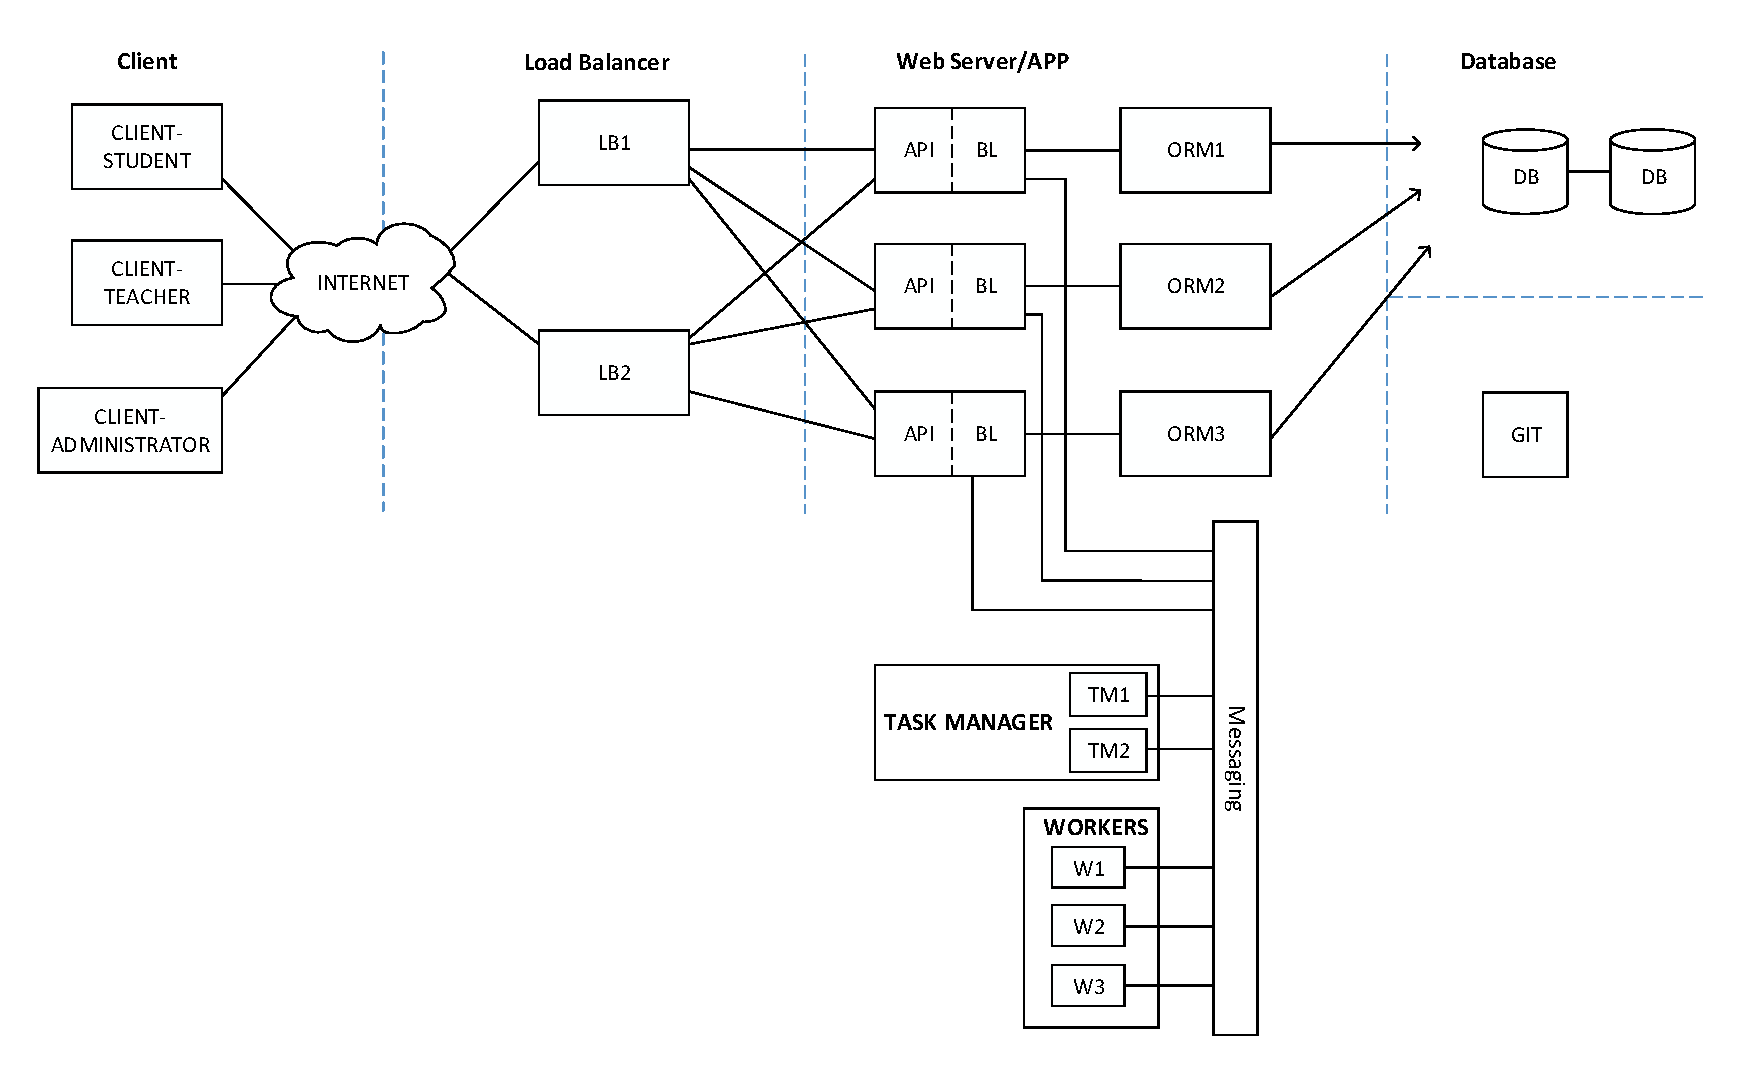
\includegraphics[height=0.95\textwidth]{figures/atfogo_rendszerterv_teljes.pdf}
		\caption[Conceptional System Design]{Conceptional System Design}
		\label{fig:conceptional-system-design}
	\end{figure}
\end{landscape}

\section{Scalability}\label{scalability}

\newparagraph{Client}
To mitigate the scalability issue, the client's code will run in a web browser for every user. This way, resources for the client's code are provided by the user as he opens the web portal in a web browser.
 
\newparagraph{Web Server}
If there were not any load balancer between the client and the web server, then one server would get every request. With thousands of users this could lead to overloads and raise the response time. With a load balancer, the requests will first arrive to the load balancer. The load balancer will decide which web server will handle that request and forward it to that web server. The choice depends on the client module, request type and the web servers' load. The load balancer's purpose is to avoid overload and minimize the response time.


 
 \section{Data Security}
 Both the back end and the front end are divided into three big modules: student, teacher and administrator. 

 \newparagraph{Web Server}
 This gives us the option to run the different modules on different computers or virtual machine instances.
 
 \newparagraph{Client}
 This ensures that one module's source code is not enough to deduce the available data, e.g., the student module will not include some API routing rules, that are included in the teacher module and the administrator module.
 

\section{Entity–Relationship Model}
\label{ER-model}

A data model describes the structures in which the database stores the data. The \emph{Entity-Relationship model} is a formal notation system, that describes the data structure with entity sets and the relationships sets~\cite{adatb}.

This data model is different from the old portal's data model, because it supports the followings:

\begin{itemize}
	\item more than one course,
	\item stores data for more than one semester, and
	\item can manage repeated classes,
\end{itemize}
 
The project's model uses Chen's notation. About 65 percent of the model was created by me, 35 percent of it was created by József Marton and it was finalized by the team. The attribute list is documented in \refstruc{attribute-list}.

The main entities are the followings:

\begin{itemize}
	\item \textbf{Appointments:} An appointment connects the student groups with a date and a location.
	\item \textbf{Courses:} The courses, that are managed with the new portal.
	\item \textbf{Deliverables:} The things to be submitted by the students (e.g. homework).
	\item \textbf{Deliverables/Repositories:} A special type of Deliverables that is to be submitted through a repository.
	\item \textbf{Deliverables/Files:} A special type of Deliverables that is to be submitted as a file upload.
	\item \textbf{DeliverableTypes:} Describes the type of the submitted homework, e.g. documentation, source code. 
	\item \textbf{Evaluator:} A many-to-many relationship between the ExerciseTypes and the Staffs. It describes which exercise type is being evaluated by a staff member.
	\item \textbf{Events:} An educational event is a class with a date for a particular student to participate.
	\item \textbf{EventTypes:} An event can be any type of class: lecture, laboratory or seminar. The Software Laboratory course has only laboratories, but in case of using it with other courses, other type of classes will be supported too.
	\item \textbf{ExerciseCategories:} Describes the type of the laboratory: DBMS, SQL, JDBC, XML technologies in databases or SOA.
	\item \textbf{ExerciseTypes:} Describe the topic and the language of the exercises. 
	\item \textbf{RegisteredStaffs:} A many-to-many relationship between the Semesters and the Staffs. It describes the staff member's role in the semester.
	\item \textbf{RegisteredStudents:} A many-to-many relationship between the Semesters and the Students. It describes which Neptun course the student registered for in the semester.
	\item \textbf{Semesters:} An instance of the course in a particular academic term.
	\item \textbf{StudentGroups:} In Software Laboratory 5 the students are assigned to different groups. A group has one demonstrator and about 20 students.
	\item \textbf{Users:} People, who use the portal during a semester.
	\item \textbf{Users/Staffs:} A type of user, who is not a student. This user can be an administrator and/or a demonstrator and/or an evaluator.
	\item \textbf{Users/Students:} A type of user, who attends the laboratories and solves a list of tasks.
\end{itemize}

This data model is not final yet, because the other modules and the back end are still under development. 

\begin{landscape}
	
	\begin{figure}[!htbp]
		\centering
		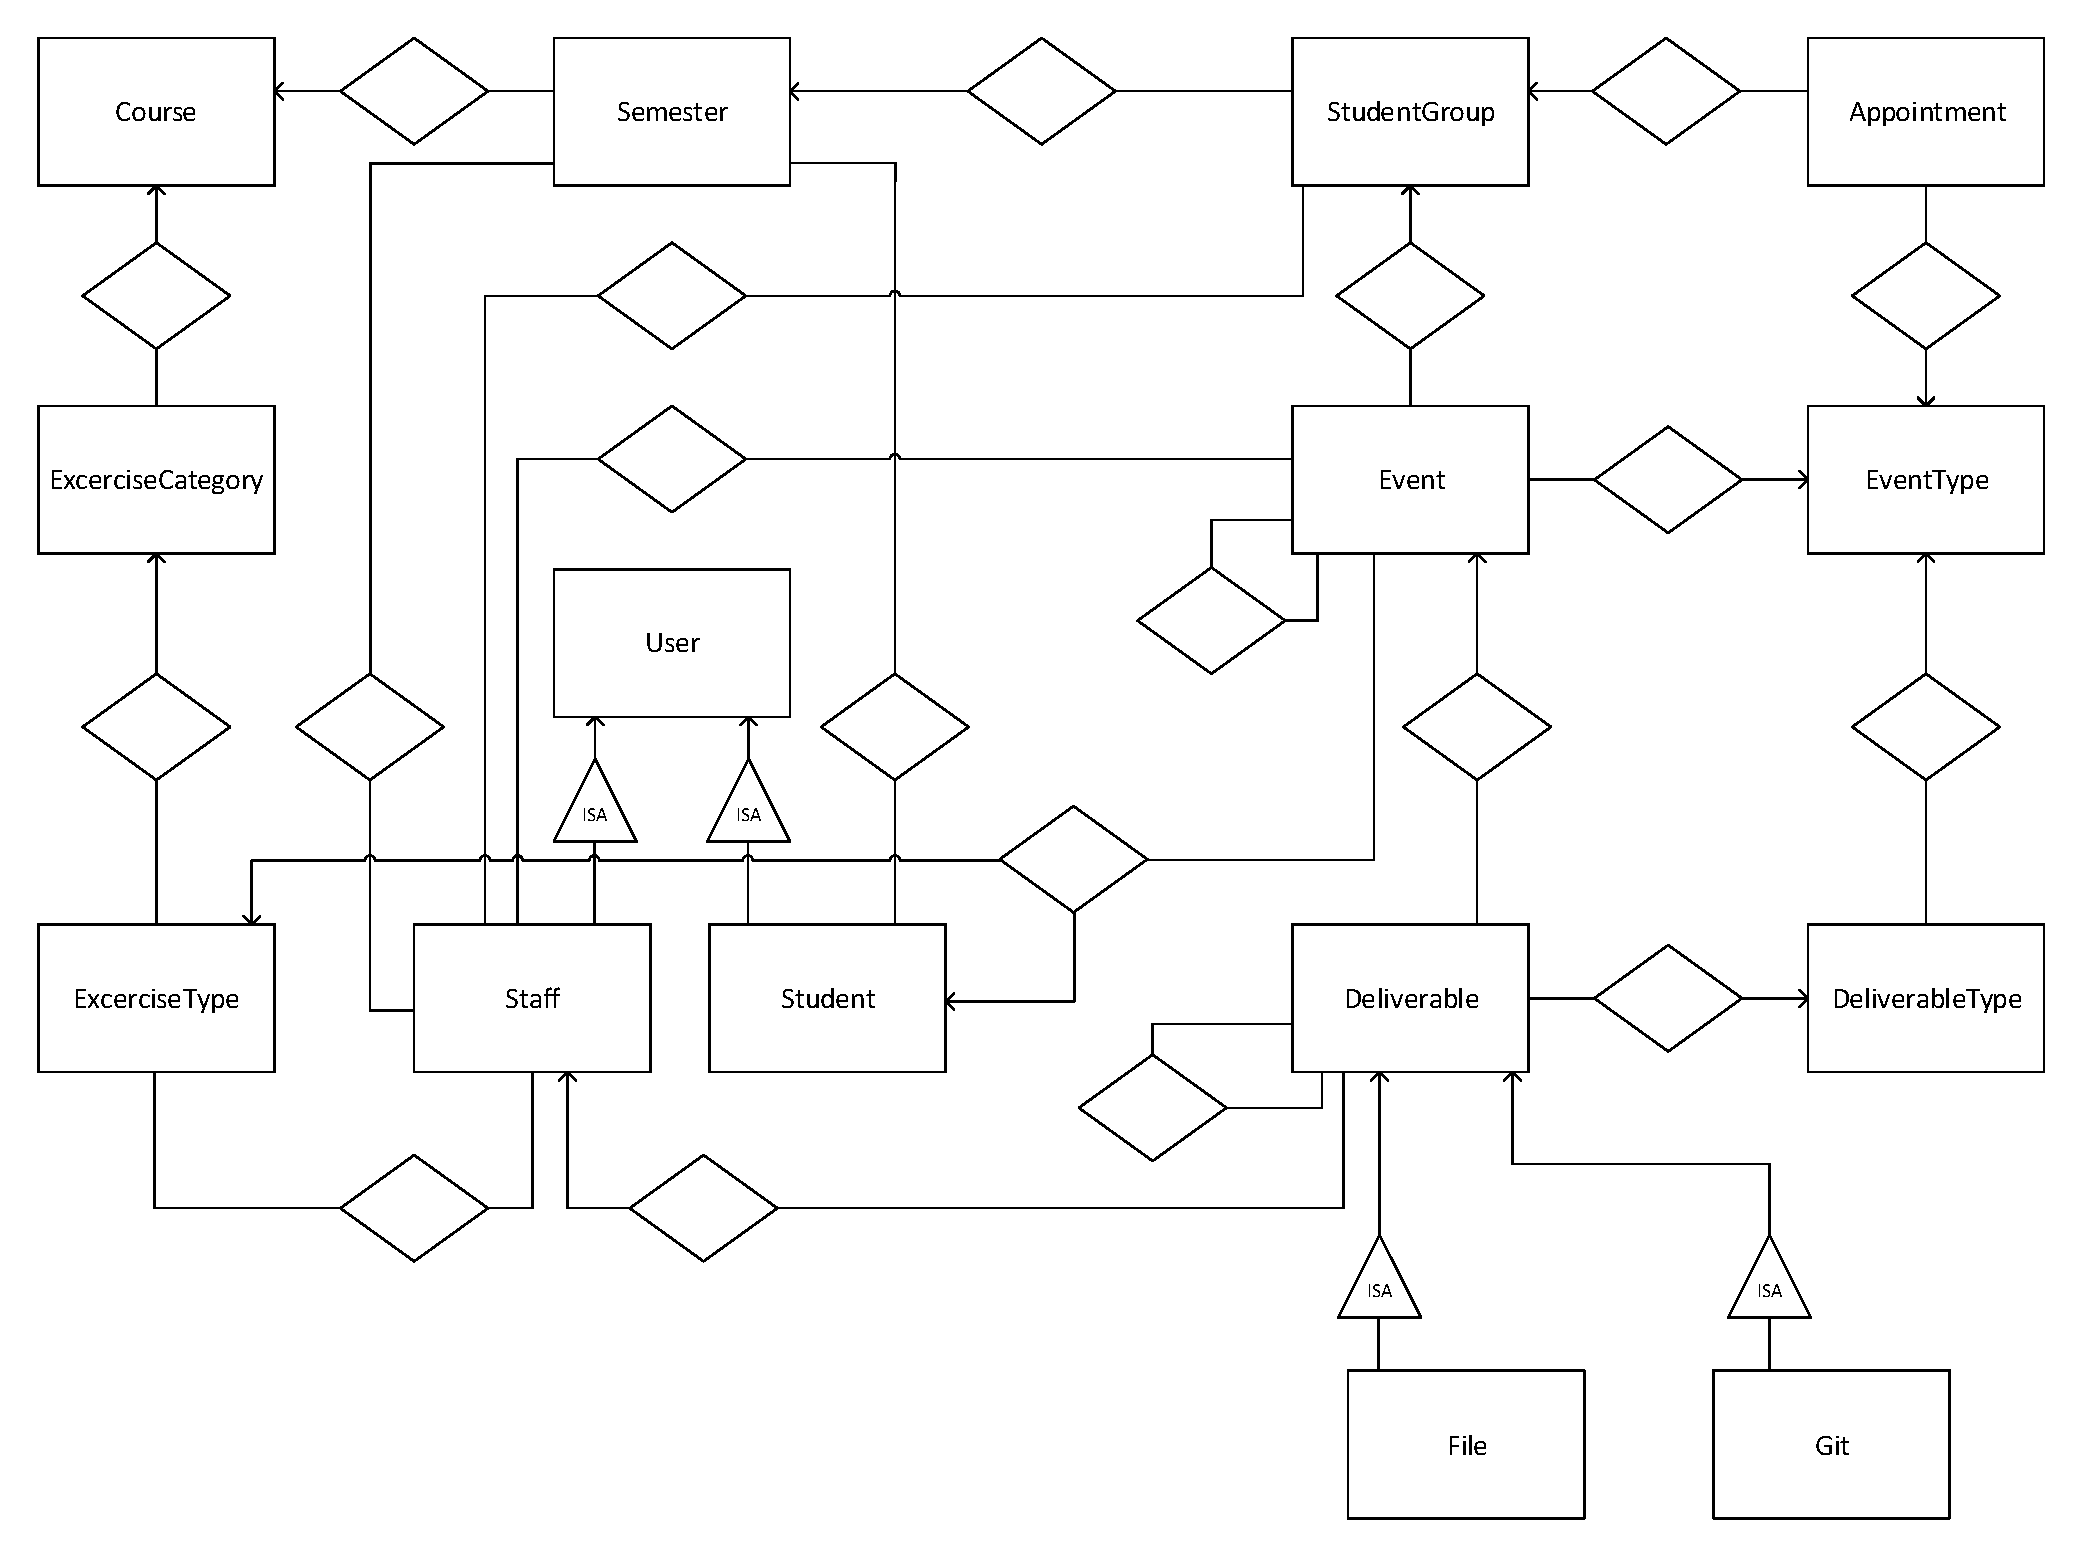
\includegraphics[width=1.3\textheight]{figures/ER.pdf}
		\caption[Entity–relationship model]{Entity–relationship model}
		\label{fig:er}
	\end{figure}
\end{landscape}




	
	\chapter{Graphic Design}

In this thesis I present the implementation of the student module. In the student module I will implement the following features in priority order:
\begin{enumerate}
	\item see general information about the classes
	\setcounter{enumi}{0}
	\item see the results
	\item list of commits and tagging a commit as final version
	\setcounter{enumi}{1}
	\item set new password, e-mail and SSH public key
	\item summarized view of student's grades
\end{enumerate}

The features with priority level 1 are mandatory, because without these features the portal will be useless for the students.

The features with priority level 2 are important, but the portal is not useless without it. The students can still tag a commit with a Git client, or merge the final commit with the master branch to make it the master branch's last commit. 

The features with priority level 3 are not important, but can be useful for students. The portal is useful without this feature, because the students can check their results on the educational event's page.

In \refstruc{7-test} I will test the features with priority level 1 and 2.


\section{Design Sketches}
To be able to draw design sketches, we need to know when will a user login to use the Educational Support System and what kind of information is he looking for. As a student, there are 5 possible scenarios:

\begin{enumerate}
	\item Before a laboratory
	\begin{itemize}
		\item To get information about the laboratory
		\begin{itemize}
			\item When will it be
			\item Where will it be
			\item Who will be the teacher
		\end{itemize}
		\item To read general information about the course
	\end{itemize}
	
	\item During a laboratory
	\begin{itemize}
		\item To upload an SSH public key
		\item To get his Git remote URL
	\end{itemize}
	
	\item After a laboratory, before the deadline for submitting the homework
	\begin{itemize}
		\item To see the date of the deadline
		\item To see how much time is left until the deadline
		\item To see the pushed branches, commits and tags
		\item To tag a commit as final version
	\end{itemize}
	
	\item After a laboratory, after deadline
	\begin{itemize}
		\item To check his grades
		\item To check his reviews
		\item To check the evaluator's name
	\end{itemize}
	
	\item Other scenarios
	\begin{itemize}
		\item To set a new e-mail address
		\item To set a new password
		\item To change his mailing list subscription
		\item To change his e-mail notification subscription
		\item To see a summarized table of his grades
	\end{itemize}
	
\end{enumerate}

With the scenarios and list of actions, we can see how many pages is needed for the student modules and how many states will one page have. 

\emph{Before laboratory:} For these information I will use only labels \see{fig:before}.

\emph{During laboratory, after laboratory and before deadline:} For the information, like deadline and entry test grade I will use labels. For the list of commits I will use a dropdown menu. When the page is loaded, the last final commit will be the chosen one. If the user did not chose a final commit before, the last commit in the master branch will be the chosen one \see{fig:during}.

\emph{After laboratory and after deadline:} For these information I will use labels. The reviews can be long, and I want to keep the design simple. Because of this, there will be a size limit for the label on the view, and the rest of the text will be hidden with an ellipsis. The user can click on the text to show the rest of the review in a pop up window \see{fig:after}.

\emph{Other scenarios:} The new e-mail address, password and SSH public keys will have input fields. The subscription will be changeable with check boxes \see{fig:settings}. The summarized view will be a simple table with the grades in it \see{fig:results}.

\emph{Menu:} Because the user is looking for a specific set of information, the page will only contain the important information, and the previous, but still relevant information will be accessible with tabs on the laboratory page. To be able to switch between the pages, I will use a navigation bar on the top of the page. The bar will have the logo of the portal and one button for each pages.

I drew sketches \see{appendix-design-sketches} for every state with placeholder data. 

\section{Design template}

To show only a specific set of information I have decided to use a minimalist design. A minimalist design is a clear design, focusing on typography, space, color and basic design elements. This way the portal will show as much information as the user needs with as few elements as possible. 

To look for templates and ideas I read the Designmodo blog~\cite{Designmodo} and checked all the popular websites, e.g., Facebook, Github, Twitter and Medium. Designmodo also have purchasable website builders, like Slides~\cite{Designmodo-slides}, but I prefer the simple design of the Bootstrap elements~\cite{Bootstrap}. 

Bootstrap is a free and open source HTML, CSS and JS framework to create responsive design. It was originally a part of Twitter as Twitter Blueprint, but in 2011 it was released as an open source project. Bootstrap contains elements for responsive web design and mobile design. Bootstrap 4 alpha was launched in August 2015 alongside with a new side project, Official Bootstrap Themes~\cite{Bootstrap-themes}. Bootstrap Themes are purchasable redesigned collections of Bootstrap components with new components and plug-ins. Although I really like these themes, I will use the free components, because it does not worth buying any theme if I will change some parts of the included components. 

\subsection{Colors}

After deciding what kind of design framework will I use, I had to chose the colors of the portal. Both the Budapest University of Technology and Economics~\cite{BME-Arculat}~\cite{BME-Arculat-Intranet} and the Faculty of Electrical Engineering and Informatics~\cite{VIK-Arculat}~\cite{VIK-Arculat-PDF} have their own Visual Identity Guidelines. A visual identity guideline contains the description of which color is the official color of the institution and in what kind of text which fonts and why that font should be used.

I consulted with my advisor, Sándor Gajdos and he told me that I should not follow any of these visual identity guidelines. Following any of the strict guidelines can be a problem in the future, if anyone would like to use this portal for another course that does not belong to the faculty or the university. Based on a subjective opinion I have decided to use green as the main color of the portal. I used the Google Color palette~\cite{google-color-chart} to choose a nice green, changed it a bit, and I got the final color, \#2a623d.

\newpage
\section{Final Graphical Design}

\begin{figure}[!ht]
	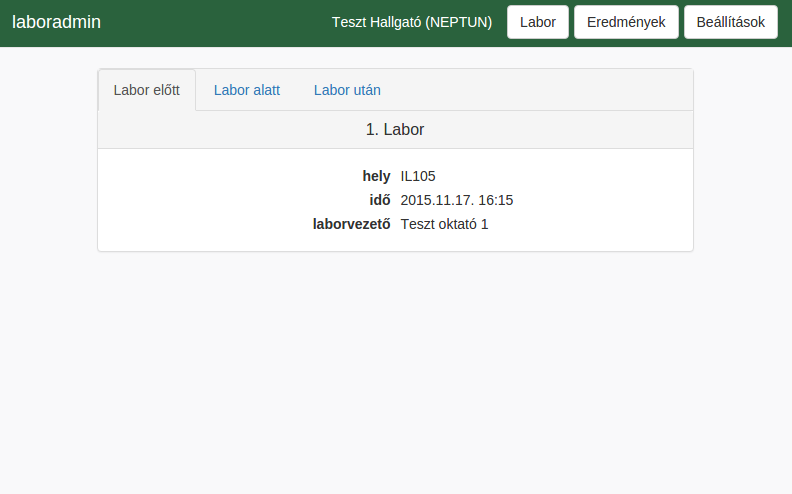
\includegraphics[width=\textwidth]{figures/design/labor_elott.png}
	\caption{Before laboratory}
	\label{fig:before}
\end{figure}

\begin{figure}[!ht]
	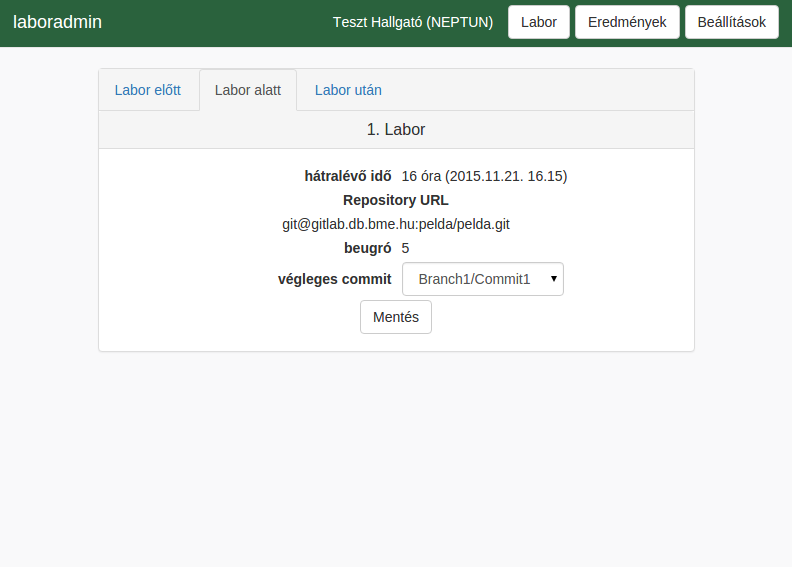
\includegraphics[width=\textwidth]{figures/design/labor_alatt.png}
	\caption{During laboratory}
	\label{fig:during}
\end{figure}

\begin{figure}[!ht]
	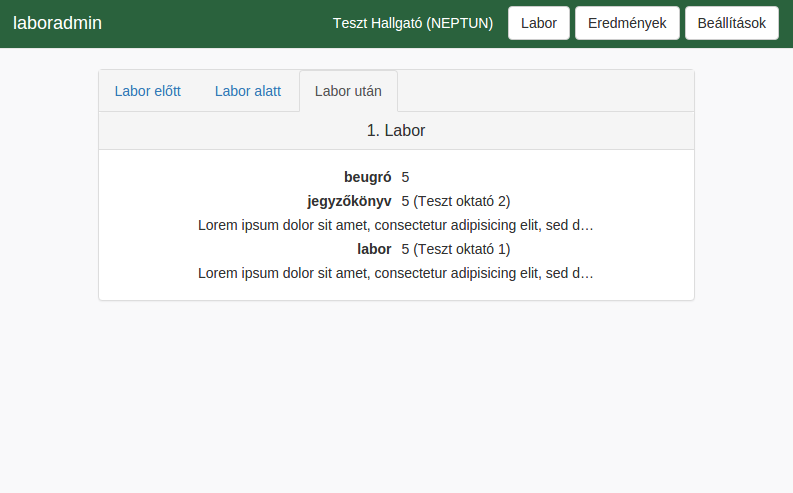
\includegraphics[width=\textwidth]{figures/design/labor_utan.png}
	\caption{After laboratory}
	\label{fig:after}
\end{figure}

\begin{figure}[!ht]
	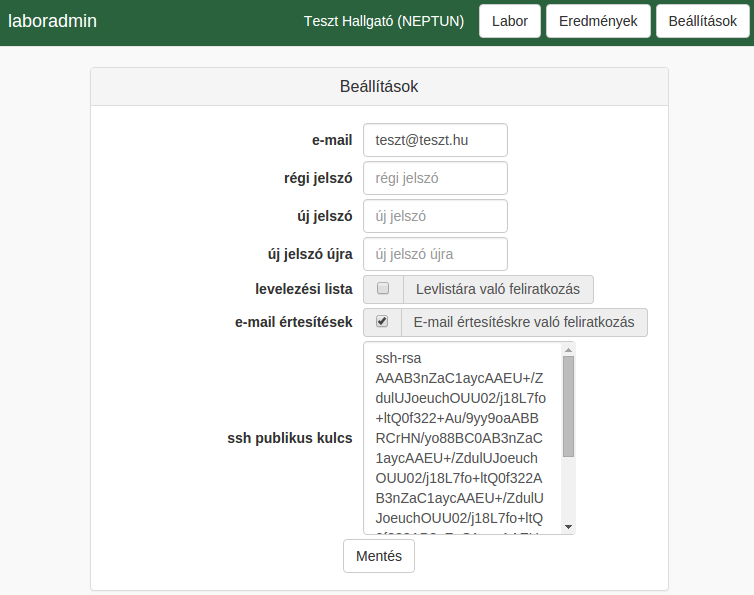
\includegraphics[width=\textwidth]{figures/design/beallitasok.png}
	\caption{Settings}
	\label{fig:settings}
\end{figure}

\begin{figure}[!ht]
	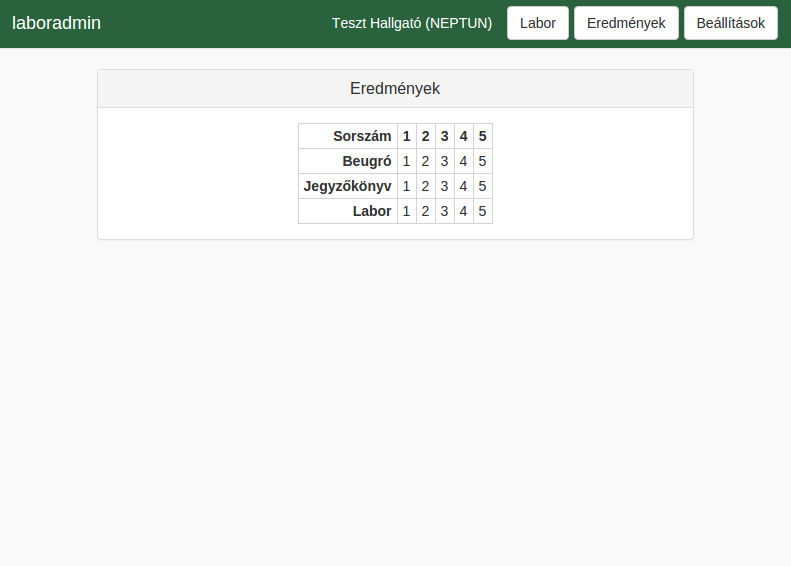
\includegraphics[width=\textwidth]{figures/design/eredmenyek.png}
	\caption{Summarized results}
	\label{fig:results}
\end{figure}

\todo{popup screenshot}

\todo{életlenséggel valamit csinálni kell, hogy fog ez kinézni nyomtatva?}
	\chapter{Implementation}\label{implementation}

The team has decided, that the portal is an open source project. The source code is available on GitHub~\cite{Github-student-frontend}~\cite{Github-backend}. This offers an opportunity for new students and staff to contribute in the project. 

\section{Version Control}
GitHub~\cite{github} is an online Git repository service. Git is a version control system. In a new commit, it stores snapshots of the file system. If a file did not change, then Git links it to the previous version~\cite{git}. GitHub offers private and public repositories too. In this project we use public repositories and the Git Workflow~\cite{git-workflow}. 

\subsection{Git Workflow}
When many developers work on the same project, their aim is to keep the master branch clean. A branch is a pointer to one of the commits (snapshots). The default branch is the master branch. To keep the master branch clean, developers can create a new branches. While developing a feature, the developer commits into a second branch. These changes does not affect the master branch. When the feature is finished, then the developer has to merge it into the master branch. If the master branch did not change, it will move the pointer to the new commit. At this point the new branch can be deleted, because the master branch points at the same commit~\cite{git-workflow2}.

If the master branch changed before, Git can do a three-way merge between the common ancestor, the last commit in the master branch, and the last commit in the second branch. Git can do this automatically, if a same part of a same file is not changed. In that case the developer can either accept one of the files or merge them by hand~\cite{git-workflow2}.

\section{Used Software Tools and Open Source Projects}
The front end uses the following open source projects and software tools:

\begin{itemize}
	\item \textbf{API Blueprint:} API Blueprint~\cite{api-blueprint} is an open source project, that gives me the option to write my specification in Markdown. I use it to describe the contract between the back end and the front end.
	\item \textbf{Bootstrap:} Bootstrap~\cite{Bootstrap} is a free and open source HTML, CSS and JS framework to create responsive design. I use it as a template for the portal's design.
	\item \textbf{Cucumber:} Cucumber~\cite{Cucumber} is a software tool to run automated tests with user stories written in the Given When Then convention. 
	\item \textbf{Drakov:} Drakov~\cite{drakov} is a mock server tool, that implements API Blueprint specifications. I use it as a mock server for the features, that are not provided by the back end yet.
	\item \textbf{GitHub:} GitHub~\cite{github} is an online Git repository service. The project's source code is available on GitHub.
	\item \textbf{Gulp:} Gulp~\cite{gulp} is a software tool to automatize tasks. I use it to concatenate and minimize files, transform HTML-like syntax in JavaScript files and move them to another directory and then to start the mock server.
	\item \textbf{Mithril:} Mithril~\cite{Mithril} is a small JavaScript MVC framework. The front end is implemented in Mithril.
	\item \textbf{JSLint:} I used the JSLint~\cite{jetbrains-jslint} code verifier plugin to verify that my JavaScript codes match the coding rules~\cite{js-conventions}.

\end{itemize}

This thesis and all the documents for this project were written in \LaTeX~\cite{latex}. \LaTeX is a markup language to create scientific documents. A TeX distribution produces the PDF output. All the diagrams were made by me in Microsft Visio 2013~\cite{visio}. Visio is a part of the Microsoft Office and is an application to create diagrams. Visio is free for students via DreamSpark~\cite{msdnaa}. For developement, I used IntelliJ IDEA~\cite{intellij-idea}, that is free for students.


\section{Method of Implementation}
During implementation I used HTML, CSS and JavaScript to create the web application. For deployment I used a gulp script written by me \see{gulp}. 

HTML is a standard language to create websites. CSS describes the style of the HTML elements. The styles are binded to the elements within the class attribute. JavaScript is a script language to make websites interactive. Web applications use JavaScript for AJAX requests and event action handling. 

\newparagraph{HTML}
As the first step I created a basic HTML page. An HTML page has a head and a body section. All the meta data belong to the head section, and anything I want to display on the page goes to the body section. \label{html-impl}

In the \emph{head section} I included a charset option and set it to utf-8 for Unicode character encoding. I added one more important meta data, the \emph{http-equiv=''x-ua-compatible''}. I use this meta tag to force Internet Explorer to render in the highest available mode~\cite{IE10-microsoft}~\cite{IE10-html5-boiler}. This solves the problem, that Internet Explorer wanted to open the website in IE10 Compatibility Mode. I also included a title and linked the main CSS file in the head section.

In the \emph{body section} I created an empty div with an id attribute. The pages are rendered into this div. To make sure that JavaScript can render elements into this div, I included the JavaScript code after the closing tag of this div.

\newparagraph{CSS}
As the main CSS file I concatenate the Bootstrap CSS file with my own CSS file, called \mbox{\emph{laboradmin.css}}. During concatenation I had to make sure that my CSS code will be after the Bootstrap code. This is important, because in CSS the last style rules overrides the previous ones. The Bootstrap CSS file contains the basic Bootstrap component styles. In the \mbox{\emph{laboradmin.css}} file some parts of the Bootstrap CSS are overwritten, to make the components to have a different appearance than the basic Bootstrap appearance, e.g., font colors, background colors and border visibility.

\newparagraph{JavaScript}
This module contains the following JavasScript files: 
\begin{itemize}
	\item the shim file, because Mithril relies on some features what are not part of the previous Internet Explorer versions,
	\item the Mithril framework's minimized JavaScript code,
	\item the Moment~\cite{moment} framework's minimized JavaScript code,
	\begin{itemize}
		\item I use this framework to calculate the time difference between the current time and the deadline.
	\end{itemize}
	\item the Bootstrap JavaScript file, because some components require it,
	\item jQuery, because Bootstrap depends on jQuery, and
	\item my JavaScript files.
\end{itemize}

During developement for the sake of maintainability, I separated my JavaScript files based on if it is a part of the model's, the controller's or the view's code. 

I use MSX in my \emph{view} codes. To make the inline HTML-like syntax more simple, I created different widgets, and use them as HTML tags. The widgets are separated in different directories based on the page that uses the widget. To build a page the followings are needed: 
\begin{itemize}
	\item a page, that contains the menu and the panel,
	\item a panel, that contains all the widgets, and
	\item the widgets, that contain the basic HTML elements.
\end{itemize}

The MSX transformer converts this HTML-like syntax into Mithril JavaScript code during the concatenation. In the HTML-like code, I add classes for every element and ids and names for some element. These class attributes will make the element's style look equal. Every class's style is defined in the CSS files. The names and ids helps finding HTML elements for event handlers and during testing.

The \emph{controllers} are the communication bridges between the model and the views. The controllers have helper methods to get the necessary data from the model, or send data to the model and to change the behavior of the elements, e.g. disable buttons. The view uses these helper methods to bind data or event listeners to the elements.

Because I did not want more dependencies I have decided to implement a simple JavaScript class as the \emph{model}. The model loads the necessary data from the server and stores it. The model can also send data to the server. All data flow between the model and the server go through a marshalling module for conversion.

During deployment I concatenate all the JavaScript files to one file and minimize it. This leads to as few requests to the back end as possible and improves the performance. The website will only download one HTML file, one CSS file and one JavaScript file.

\section{Final Version}
I have uploaded the code to GitHub. The commit, that is presented in this thesis is tagged with \emph{thesis-final2}~\cite{Github-final}.

	\chapter{Test}
\label{7-test}

To test the application I used Cucumber with user stories for acceptance tests with Zombie as a headless browser and Istanbul for code coverage testing. I also used a mock server to get mock data during testing, because the back end modules are not finished yet.

\section{Communication Interfaces}
As I mentioned in \refstruc{api-blueprint}, I used the API Blueprint specification to define the communication interfaces. The files are available on Github~\cite{Github-blueprint}. Mock server usage is described in \refstruc{mock-server-usage}.


\section{Testing}
\subsection{Acceptance Tests}
An acceptance test validates that this is the software or feature the customer wanted. I wrote user stories \see{spec-user-story} for the features I wanted to test based on the user stories I wrote during the specification phase~\cite{szofttech}.

\subsubsection{Cucumber}
\label{cucumber-test}

I used Cucumber \see{spec-cucumber} to implement acceptance tests. I used the instructions on the Cucumber website to start the implementation~\cite{github-cucumberjs}. A Cucumber test requires the following files:

\begin{itemize}
	\item \textbf{Features Files:} The user stories are stored in feature files.
	\item \textbf{Support Files:} These will be run before each scenario to create the test environment. In my case it creates a headless browser. One example is included on the Cucumber website, but that does not work. I implemented my own support file.
	\item \textbf{Step Definitions:} These are the implemented feature steps. I generated the functions with a JetBrains plugin~\cite{jetbrains-cucumber} and implemented the logic for every step. 
\end{itemize}

\subsubsection{Zombie}
I wanted to use a browser to test the client's JavaScript code. My first choice was Selenium~\cite{selenium} with a Google Chrome browser, but the tests were slow. To solve this issue I have decided to use a browser without a user interface. I chose Zombie, because it was recommended on the Cucumber website.

Zombie~\cite{zombie} is lightweight framework, that implements a browser without a user interface. It also supports assertions, that makes it possible to text field comparison and HTML element existence testing easier, and pipelines to log the outgoing requests from the Zombie browser. 

\subsection{Code Coverage Tests}
A coverage test measures which functions, statements, lines were executed~\cite{szofttech}. I tested which user stories w

\subsubsection{Istanbul}
Istanbul~\cite{istanbul} is a code coverage software tool for JavaScript. It checks coverage for:

\begin{itemize}
	\item \emph{Function:} number of functions, that have been called.
	\item \emph{Statement:} number of statements, that have been executed.
	\item \emph{Branch:} Number of branches, that have been executed.
\end{itemize}

\subsection{Automatized Tests}
First follow the instructions in \refstruc{deployment}, then start the mock server. Use the following command to run the Cucumber tests:

\monospace{npm test}

I have implemented 14 scenarios and 91 steps. Use the following command to run the Cucumber tests with code coverage:

\monospace{npm test \texttt{-{}-}coverage}

The following features were implemented:

\begin{enumerate}
	\item see the general information about the classes
	\setcounter{enumi}{0}
	\item see the results
	\item see a list of commits and tagging a commit as final version
	\setcounter{enumi}{1}
	\item set new password, e-mail and SSH public key
	\item summarized view of student's grades
\end{enumerate}

As I mentioned in \refstruc{design-specification}, I tested the features with priority levels 1 and 2.

During the testing I was comparing the HTML elements' texts with the example data that came form the user story and the elements' existence. If a label contains a date, I used a regex for pattern matching:

\monospace{(\textbackslash d{4})\textbackslash.(\textbackslash d{2})\textbackslash.(\textbackslash d{2})\textbackslash. (\textbackslash d{2}):(\textbackslash d{2})}

Because I cannot test features, that needs to change the database, without a real back end, I tested for outgoing requests. If there was an outgoing request for the specific URL, the test passed. This  also gave me the option to test for not outgoing requests. For example, to set a new password, the user has to fill out three input fields: old password once and new password once. If any of these fields were empty, or the new password fields do not contain the same password, then the client should not send a request to the server. I wrote scenarios to all 8 possible states. These tests will change when the back end modules will be implemented.

In this phase the client has a save button on the settings page. As a future improvement in the next version, I will set the save mechanism to the fields on change events. Because of this the server only requires two parameters in the HTTP request's body: mailing list subscription and notification subscription. These parameters will always have a valid value, because the check box fields return a boolean value, either true or false.

\subsubsection{Test Results}
In behavior-driven development the developer implements first the tests, that fail. Then the developer implements the missing features, until all the tests for that feature passes. After running the tests, all scenarios and steps passed. This means that all the features, that are prescribed in the functional specification were implemented and tested. The coverage summary for the test Javascript files are almost 100\%. The branch summery is only 55 \%, because the lines, that contain a command to send an error did not run.

\begin{figure}[!ht]
	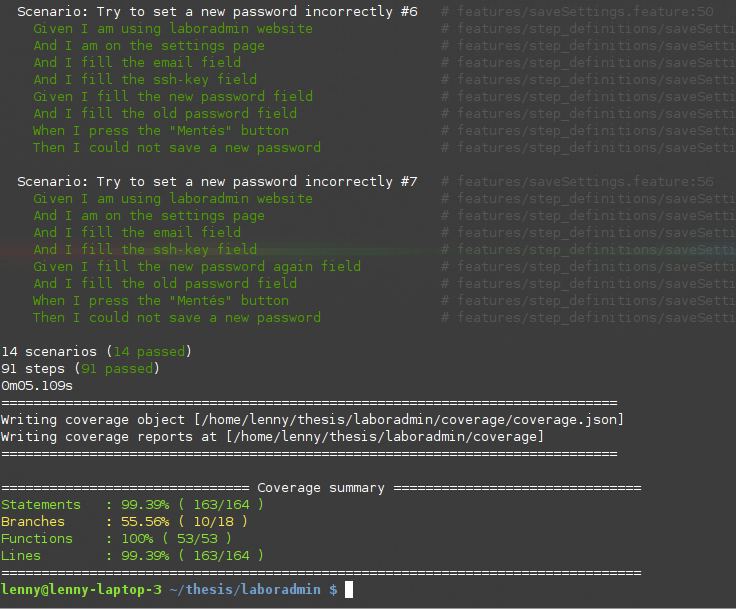
\includegraphics[width=\textwidth]{figures/test-result.png}
	\caption{Part of the Tests' Output}
	\label{fig:test-results}
	\end{figure}


	\chapter{Deployment}

\bence{Megy az Windowson is, irreleváns a Linux rész}

I wrote a gulp script on Linux to automatize the deployment. This script creates the three downloadable files from the source codes.

\section{Gulp}
\label{gulp}

Gulp is a software tool to automatize tasks. I use it to concatenate and minimize files, transform HTML-like syntax in JavaScript files and move them to another directory and then to start the mock server.

To install gulp on Linux, I used the npm package manager from a terminal, that was opened in the project's root folder. Gulp can be installed as a global package with the following command:

\bence{Hívható parancsokat és konzolos kimeneteket nem dőlt betűvel szokás
  megjeleníteni.  Monospace betűtípust használj és legyen egyértelmű, hogy
  melyik rész a meghívott parancs, mit kell root és mit lehet sima
  felhasználóként meghívni.  És az is legyen egyértelmű, hogy mi a kimenet.  Ha
  az túl hosszú, akkor illik rövidíteni}

\emph{npm install -g gulp}

\subsection{Gulp Plugins}

I use the following Gulp plugins:

\begin{itemize}
	\item drakov
	\item gulp-concat
	\item gulp-minify-css
	\item gulp-minify-html
	\item gulp-plumber		
	\item gulp-uglify
	\item gulp-util
	\item msx
	\item through2
\end{itemize}
	
Use the following code to install plugins:

\emph{npm install [plugin1 plugin2 plugin3]}

\subsection{The Gulp File}
The client's gulp file is added in the root directory. 

First gulp uses the msx plugin, to transform the HTML-like syntax in the JavaScript files, then concatenates them. The concatenated JavaScript file is minimized and moved to the \emph{dist} folder. I used the MSX plugin's example code for the msx transformation task~\cite{gulp-msx-example}. Then gulp minimizes the HTML file and moves it to the \emph{dist} folder. At last the CSS files are concatenated, minimized and the minimized file is moved to the \emph{dist} folder.

Use the following command to run it:

\emph{gulp}

The final three files are in the \emph{dist} folder. These files will be downloaded from the server, when a user opens the portal in a browser.

	\chapter{Conclusion}\label{conclusion}

In this chapter I summarize my work and I introduce the future plans.

\section{Summary of my Work}
I achieved the followings:
\begin{itemize}
	\item wrote the new portal's functional specification,
	\item compared three JavaScript frameworks and chose one for implementation,
	\item created the front end system design based on the behavior of the chosen,
	\item created the database schema with József Marton,
	\item created a high level system design with Bence Golda,
	\item designed the communication between the client and the server,
	\item implemented the front end student module,
	\item tested the student module with acceptance tests, and
	\item documented the deployment process.
\end{itemize}

\section{Future Work}
After this thesis I will continue to work on the front end modules and the system's design. Although I have created a database scheme and the system design, they are still in development. The front end modules will be implemented first, and then I will work more on the graphic design if the team is not satisfied with it. Because the project is still under development, it is possible, that the first official version, what is going to be used in the Software Laboratory 5 course from February 2016, will be different from the one presented in this thesis.

\pagenumbering{roman}
\setcounter{page}{\value{romanPage}}


% Acknowledgements
%~~~~~~~~~~~~~~~~~~~~~~~~~~~~~~~~~~~~~~~~~~~~~~~~~~~~~~~~~~~~~~~~~~~~~~~~~~~~~~~~~~~~~~
	%----------------------------------------------------------------------------
\chapter*{\koszonetnyilvanitas}\addcontentsline{toc}{chapter}{\koszonetnyilvanitas}
%----------------------------------------------------------------------------

%Ez nem kötelező, akár törölhető is. Ha a szerző szükségét érzi, itt lehet köszönetet nyilvánítani azoknak, akik hozzájárultak munkájukkal ahhoz, hogy a hallgató a szakdolgozatban vagy diplomamunkában leírt feladatokat sikeresen elvégezze. A konzulensnek való köszönetnyilvánítás sem kötelező, a konzulensnek hivatalosan is dolga, hogy a hallgatót konzultálja.

First, I would like to thank  Bence Golda for all his help and advice and Sándor Gajdos for his mentorship, advice and continued involvement throughout this project. 

My deep  gratitude  for József Marton for offering me his office and granting me the academic support and advice throughout this challenging endeavor.  

In conclusion, I would like to acknowledge my family, my boyfriend, Lars Vandenbergh, and my friends Kálmán Tarnay, Gábor Váradi, Zoltán Czirkos, Dalma Babinszki, Dániel Stein, Ferenc and Anni  Karpati for their unconditional love, encouragement, and continuous  commitment to me both throughout my undergraduate studies  and the preparation of this thesis.


% List of Figures, Tables
%~~~~~~~~~~~~~~~~~~~~~~~~~~~~~~~~~~~~~~~~~~~~~~~~~~~~~~~~~~~~~~~~~~~~~~~~~~~~~~~~~~~~~~
%TODO your own content
	\listoffigures\addcontentsline{toc}{chapter}{\abrakjegyzeke}
	\listoftables\addcontentsline{toc}{chapter}{\tablazatokjegyzeke}


% Bibliography
%~~~~~~~~~~~~~~~~~~~~~~~~~~~~~~~~~~~~~~~~~~~~~~~~~~~~~~~~~~~~~~~~~~~~~~~~~~~~~~~~~~~~~~
%TODO your own content
	\bibliography{bib/diploma}
	\addcontentsline{toc}{chapter}{\irodalomjegyzek}

% Appendix
%~~~~~~~~~~~~~~~~~~~~~~~~~~~~~~~~~~~~~~~~~~~~~~~~~~~~~~~~~~~~~~~~~~~~~~~~~~~~~~~~~~~~~~
%TODO your own content
%	%----------------------------------------------------------------------------
\appendix
%----------------------------------------------------------------------------
%\chapter{\fuggelek}\addcontentsline{toc}{chapter}{\fuggelek}
%\setcounter{chapter}{6}  % a fofejezet-szamlalo az angol ABC 6. betuje (F) lesz
\setcounter{equation}{0} % a fofejezet-szamlalo az angol ABC 6. betuje (F) lesz
\numberwithin{equation}{section}
\numberwithin{figure}{section}
\numberwithin{lstlisting}{section}
%\numberwithin{tabular}{section}


\chapter{Data Dictionary}

The data dictionary describes the meaning of the words and terms used in the Educational Support System and the Software Laboratory 5 course.

\begin{itemize}
	\item \textbf{Administrator} A person, who is responsible for running the administration system.
	\item \textbf{Course, subject} A program of instruction in a university.
	\item \textbf{Demonstrator} A person, who teaches a group of students.
	\item \textbf{Entry test, short test, quiz} An evidence that verifies the preparedness of the student.
	\item \textbf{Entry test grade, mark} A number indicating the quality of the student's preparedness.
	\item \textbf{Evaluator} A person, who evaluates the laboratory reports.
	\item \textbf{Event, educational event} An educational event is a class with a date for students to participate.
	\item \textbf{Excercises, tasks} A list of exercises that provides experience to a student with a technology.
	\item \textbf{Laboratory} A type of class held in a computer laboratory by a demonstrator to a group of students.
	\item \textbf{Laboratory grade, mark} A number indicating the quality of the student's laboratory work.
	\item \textbf{Laboratory report, documentation} The documentation about how the student  solved the list of exercises.
	\item \textbf{Review, remark} The evaluator's assessment of the quality of the solutions and submitted materials.
	\item \textbf{Semester, term} Half of a school year, lasting about five months.
	\item \textbf{Source code} The program code written by a student to solve a list of exercises.
	\item \textbf{Student, pupil} A person, who is responsible for running the administration system.
\end{itemize}

To search synonyms and write definitions I used an online synonym dictionary~\cite{Thesaurus}, and an online explanatory  dictionary~\cite{Dictionary}.
\chapter{User Stories}
\label{user-stories}

\textbf{Feature: Student module}\\ \hspace*{1cm}
As a student\\ \hspace*{1cm}
I want to get information about my laboratories\\ \hspace*{1cm}
to know where to upload my homework\\ \hspace*{1cm}
And read the remarks of my homeworks\\ \hspace*{1cm}
And change my basic settings

\underline{Before laboratory:}

Background:\\ \hspace*{1cm}
Given a student named "Jakab"\\ \hspace*{1cm}
And his password and username are entered in the login fields\\ \hspace*{1cm}
And it is one day before the laboratory\\ \hspace*{1cm}
And a finished homework uploaded to the Git repository

Scenario: Getting information about the next laboratory\\ \hspace*{1cm}
Given I open the Laboradmin page\\ \hspace*{1cm}
When I press the login button\\ \hspace*{1cm}
Then I should see the date of my next laboratory\\ \hspace*{1cm}
And  I should see the room number of my next laboratory\\ \hspace*{1cm}
And I should see the name of my teacher

\underline{During laboratory:}

Background:\\ \hspace*{1cm}
Given a student named "Jakab"\\ \hspace*{1cm}
And his password and username are entered in the login fields\\ \hspace*{1cm}
And he is sitting at the laboratory

Scenario: Getting a Git remote URL\\ \hspace*{1cm}
Given I open the Laboradmin page\\ \hspace*{1cm}
When I press the login button\\ \hspace*{1cm}
Then I should see a Git remote URL

Scenario: Check how many hours I have left\\ \hspace*{1cm}
Given I open the Laboradmin page\\ \hspace*{1cm}
When I press the login button\\ \hspace*{1cm}
Then I should see a timer with a number between 96 and 92\pagebreak



\underline{After laboratory, before deadline:}

Background:\\ \hspace*{1cm}
Given a student named "Jakab"\\ \hspace*{1cm}
And his password and username are entered in the login fields\\ \hspace*{1cm}
And it's one day before the deadline\\ \hspace*{1cm}
And a finished homework uploaded to the Git repository

Scenario: Getting a list of Git commits\\ \hspace*{1cm}
Given I open the Laboradmin page\\ \hspace*{1cm}
When I press the login button\\ \hspace*{1cm}
Then I should see a list of branches, commits and tags

Scenario: Check how many hours I have left\\ \hspace*{1cm}
Given I open the Laboradmin page\\ \hspace*{1cm}
When I press the login button\\ \hspace*{1cm}
Then I should see a timer with a number between 24 and 0


Scenario: Marking a commit as final\\ \hspace*{1cm}
Given I open the main page\\ \hspace*{1cm}
And I see a list of branches and commits\\ \hspace*{1cm}
When I click on one of the commit in the list\\ \hspace*{1cm}
Then I should see "The commit was marked as final."

Scenario: Removing a final mark\\ \hspace*{1cm}
Given I open the main page\\ \hspace*{1cm}
And I see a list of commits\\ \hspace*{1cm}
And one commit is already marked as final\\ \hspace*{1cm}
When I click on the master branch in the list\\ \hspace*{1cm}
Then I should see "You have succesfully removed your final mark."



\underline{After laboratory, after deadline:}

Background:\\ \hspace*{1cm}
Given a student named "Jakab"\\ \hspace*{1cm}
And his password and username are entered in the login fields\\ \hspace*{1cm}
And it's one day after the deadline

Scenario: Getting my grade and review\\ \hspace*{1cm}
Given I open the Laboradmin page\\ \hspace*{1cm}
When I press the login button\\ \hspace*{1cm}
Then I should see my grade and review



\underline{Other situations:}

Background:\\ \hspace*{1cm}
Given a student named "Jakab"\\ \hspace*{1cm}
And his password and username are entered in the login fields

Scenario: Getting a summarized list of my grades\\ \hspace*{1cm}
Given I am logged in as "Jakab"\\ \hspace*{1cm}
When I press the summary button\\ \hspace*{1cm}
Then I should see all of my grades

Background:\\ \hspace*{1cm}
Given a logged in student named "Jakab"\\ \hspace*{1cm}
And the settings page is loaded

Scenario: Setting a new SSH public key\\ \hspace*{1cm}
Given I am logged in as "Jakab"\\ \hspace*{1cm}
And I have entered a new SSH public key\\ \hspace*{1cm}
When I press the save button\\ \hspace*{1cm}
Then I should see "Your settings have been saved."

Scenario: Setting a new e-mail address\\ \hspace*{1cm}
Given I am logged in as "Jakab"\\ \hspace*{1cm}
And I have entered a new e-mail address\\ \hspace*{1cm}
When I press the save button\\ \hspace*{1cm}
Then I should see "Your settings have been saved."

Scenario: Changing my subscription for the mailing list\\ \hspace*{1cm}
Given I am logged in as "Jakab"\\ \hspace*{1cm}
And I clicked the checkbox next to "Subscription for mailing list\\ \hspace*{1cm}
When press the save button\\ \hspace*{1cm}
Then I should see "Your settings have been saved."

Scenario: Changing my subscription for notifications\\ \hspace*{1cm}
Given I am logged in as "Jakab"\\ \hspace*{1cm}
And I clicked the checkbox next to "Subscription for notification"\\ \hspace*{1cm}
When press the save button\\ \hspace*{1cm}
Then I should see "Your settings have been saved."
\chapter{Design sketches}\label{design-sketches}
I didn't use a tool, because the design is not standardized, and it's easier and faster drawing by hand then by a tool.

\todo{szebben lerajzolni vonalzóval!!!!! vagy megcsinálni az egészet egy tool-lal, mert ez így csúnya}
%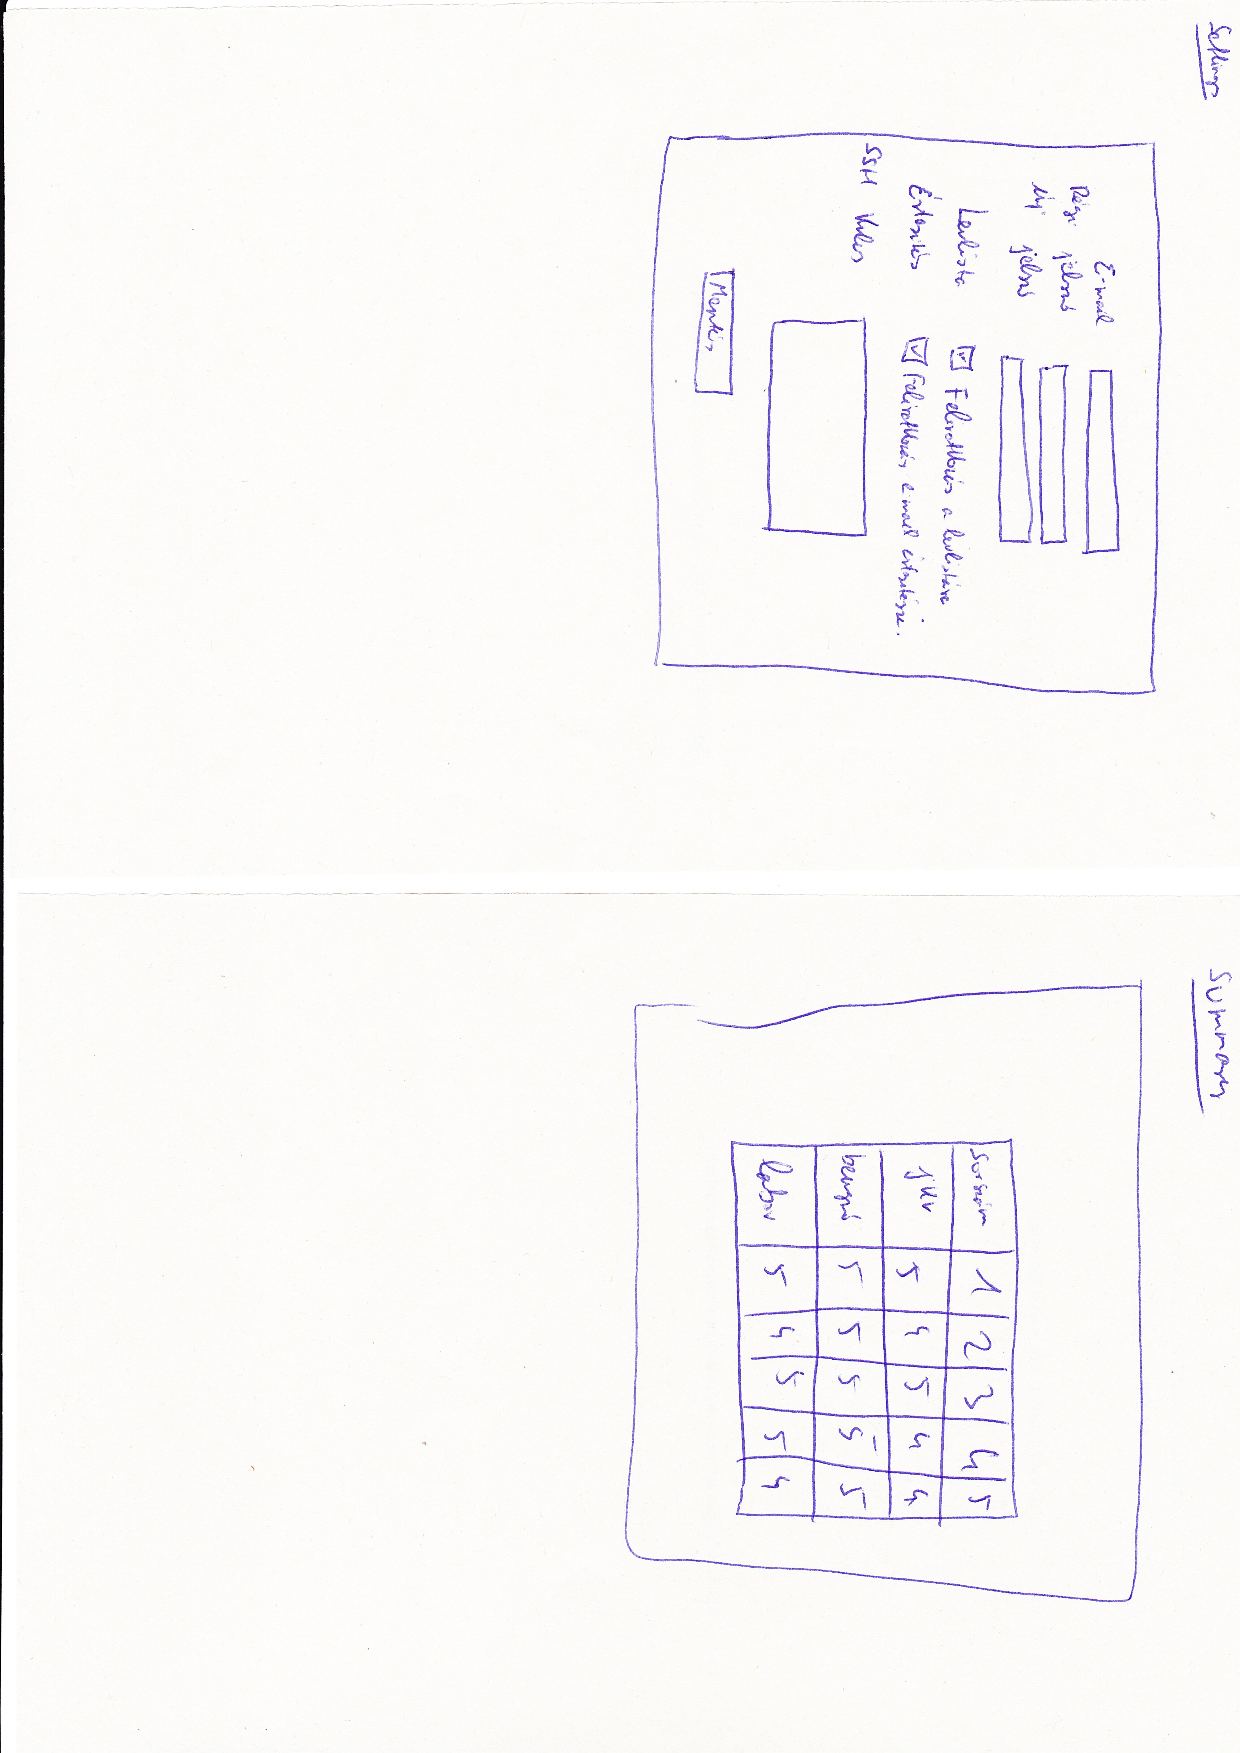
\includepdf[pages=-]{figures/sketches.pdf}
\begin{figure}[!ht]
	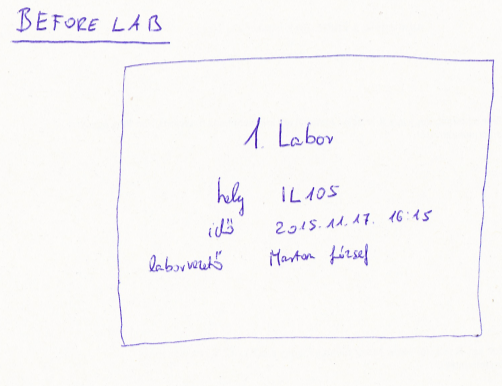
\includegraphics[width=\textwidth]{figures/sketch5.png}
	\caption{Laboratory page sketch, before lab}
	\label{fig:sketch5}
\end{figure}

\begin{figure}[!ht]
	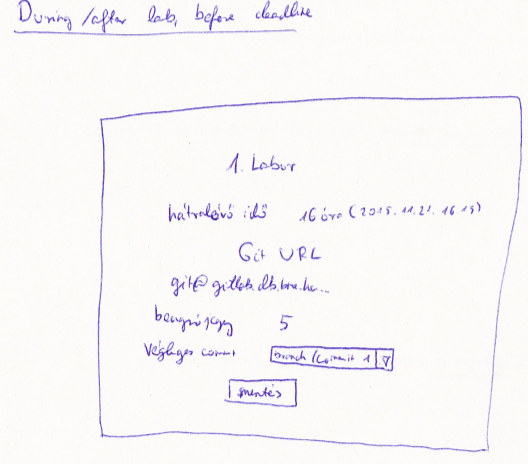
\includegraphics[width=\textwidth]{figures/sketch3.png}
	\caption{Laboratory page sketch, during/after lab, before deadline}
	\label{fig:sketch3}
\end{figure}

\begin{figure}[!ht]
	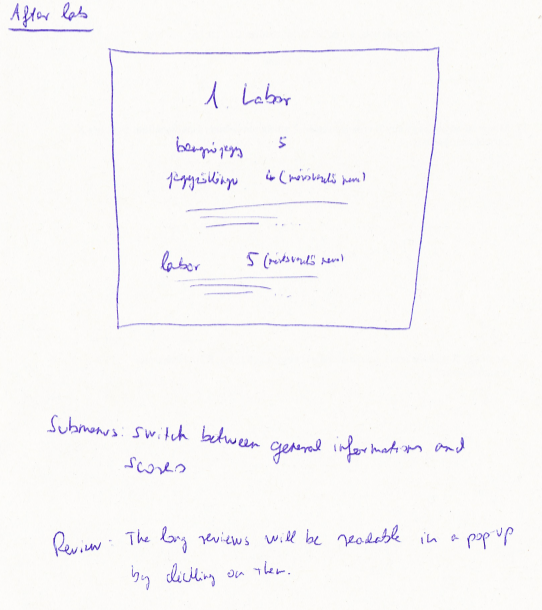
\includegraphics[width=\textwidth]{figures/sketch4.png}
	\caption{Laboratory page sketch, after lab}
	\label{fig:sketch4}
\end{figure}

\begin{figure}[!ht]
	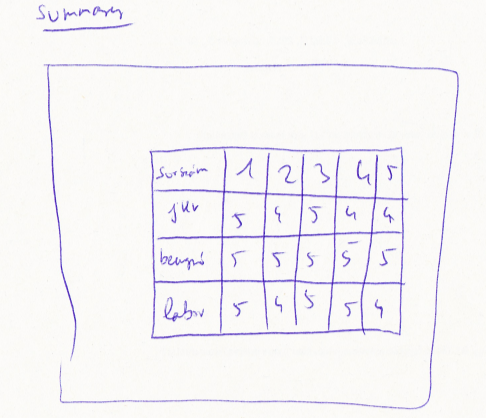
\includegraphics[width=\textwidth]{figures/sketch2.png}
	\caption{Summary page sketch}
	\label{fig:sketch2}
\end{figure}

\begin{figure}[!ht]
	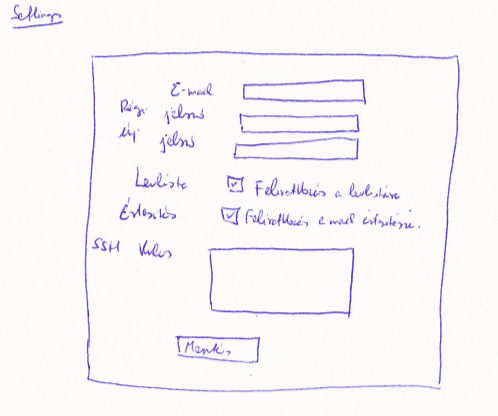
\includegraphics[width=\textwidth]{figures/sketch1.png}
	\caption{Settings page sketch}
	\label{fig:sketch1}
\end{figure}




%----------------------------------------------------------------------------
\appendix
%----------------------------------------------------------------------------
%\chapter{\fuggelek}%\addcontentsline{toc}{chapter}{\fuggelek}
%\setcounter{chapter}{6}  % a fofejezet-szamlalo az angol ABC 6. betuje (F) lesz
%\setcounter{equation}{0} % a fofejezet-szamlalo az angol ABC 6. betuje (F) lesz
\numberwithin{equation}{section}
\numberwithin{figure}{section}
\numberwithin{lstlisting}{section}
%\renewcommand\thesection{\Alph{section}}
%\numberwithin{tabular}{section}
\chapter{Data Dictionary}

The data dictionary describes the meaning of the words and terms used in the Educational Support System and the Software Laboratory 5 course.

\begin{itemize}
	\item \textbf{Administrator} A person, who is responsible for running the administration system.
	\item \textbf{Course, subject} A program of instruction in a university.
	\item \textbf{Demonstrator} A person, who teaches a group of students.
	\item \textbf{Entry test, short test, quiz} An evidence that verifies the preparedness of the student.
	\item \textbf{Entry test grade, mark} A number indicating the quality of the student's preparedness.
	\item \textbf{Evaluator} A person, who evaluates the laboratory reports.
	\item \textbf{Event, educational event} An educational event is a class with a date for students to participate.
	\item \textbf{Excercises, tasks} A list of exercises that provides experience to a student with a technology.
	\item \textbf{Laboratory} A type of class held in a computer laboratory by a demonstrator to a group of students.
	\item \textbf{Laboratory grade, mark} A number indicating the quality of the student's laboratory work.
	\item \textbf{Laboratory report, documentation} The documentation about how the student  solved the list of exercises.
	\item \textbf{Review, remark} The evaluator's assessment of the quality of the solutions and submitted materials.
	\item \textbf{Semester, term} Half of a school year, lasting about five months.
	\item \textbf{Source code} The program code written by a student to solve a list of exercises.
	\item \textbf{Student, pupil} A person, who is responsible for running the administration system.
\end{itemize}

To search synonyms and write definitions I used an online synonym dictionary~\cite{Thesaurus}, and an online explanatory  dictionary~\cite{Dictionary}.
\chapter{User Stories}
\label{user-stories}

\textbf{Feature: Student module}\\ \hspace*{1cm}
As a student\\ \hspace*{1cm}
I want to get information about my laboratories\\ \hspace*{1cm}
to know where to upload my homework\\ \hspace*{1cm}
And read the remarks of my homeworks\\ \hspace*{1cm}
And change my basic settings

\underline{Before laboratory:}

Background:\\ \hspace*{1cm}
Given a student named "Jakab"\\ \hspace*{1cm}
And his password and username are entered in the login fields\\ \hspace*{1cm}
And it is one day before the laboratory\\ \hspace*{1cm}
And a finished homework uploaded to the Git repository

Scenario: Getting information about the next laboratory\\ \hspace*{1cm}
Given I open the Laboradmin page\\ \hspace*{1cm}
When I press the login button\\ \hspace*{1cm}
Then I should see the date of my next laboratory\\ \hspace*{1cm}
And  I should see the room number of my next laboratory\\ \hspace*{1cm}
And I should see the name of my teacher

\underline{During laboratory:}

Background:\\ \hspace*{1cm}
Given a student named "Jakab"\\ \hspace*{1cm}
And his password and username are entered in the login fields\\ \hspace*{1cm}
And he is sitting at the laboratory

Scenario: Getting a Git remote URL\\ \hspace*{1cm}
Given I open the Laboradmin page\\ \hspace*{1cm}
When I press the login button\\ \hspace*{1cm}
Then I should see a Git remote URL

Scenario: Check how many hours I have left\\ \hspace*{1cm}
Given I open the Laboradmin page\\ \hspace*{1cm}
When I press the login button\\ \hspace*{1cm}
Then I should see a timer with a number between 96 and 92\pagebreak



\underline{After laboratory, before deadline:}

Background:\\ \hspace*{1cm}
Given a student named "Jakab"\\ \hspace*{1cm}
And his password and username are entered in the login fields\\ \hspace*{1cm}
And it's one day before the deadline\\ \hspace*{1cm}
And a finished homework uploaded to the Git repository

Scenario: Getting a list of Git commits\\ \hspace*{1cm}
Given I open the Laboradmin page\\ \hspace*{1cm}
When I press the login button\\ \hspace*{1cm}
Then I should see a list of branches, commits and tags

Scenario: Check how many hours I have left\\ \hspace*{1cm}
Given I open the Laboradmin page\\ \hspace*{1cm}
When I press the login button\\ \hspace*{1cm}
Then I should see a timer with a number between 24 and 0


Scenario: Marking a commit as final\\ \hspace*{1cm}
Given I open the main page\\ \hspace*{1cm}
And I see a list of branches and commits\\ \hspace*{1cm}
When I click on one of the commit in the list\\ \hspace*{1cm}
Then I should see "The commit was marked as final."

Scenario: Removing a final mark\\ \hspace*{1cm}
Given I open the main page\\ \hspace*{1cm}
And I see a list of commits\\ \hspace*{1cm}
And one commit is already marked as final\\ \hspace*{1cm}
When I click on the master branch in the list\\ \hspace*{1cm}
Then I should see "You have succesfully removed your final mark."



\underline{After laboratory, after deadline:}

Background:\\ \hspace*{1cm}
Given a student named "Jakab"\\ \hspace*{1cm}
And his password and username are entered in the login fields\\ \hspace*{1cm}
And it's one day after the deadline

Scenario: Getting my grade and review\\ \hspace*{1cm}
Given I open the Laboradmin page\\ \hspace*{1cm}
When I press the login button\\ \hspace*{1cm}
Then I should see my grade and review



\underline{Other situations:}

Background:\\ \hspace*{1cm}
Given a student named "Jakab"\\ \hspace*{1cm}
And his password and username are entered in the login fields

Scenario: Getting a summarized list of my grades\\ \hspace*{1cm}
Given I am logged in as "Jakab"\\ \hspace*{1cm}
When I press the summary button\\ \hspace*{1cm}
Then I should see all of my grades

Background:\\ \hspace*{1cm}
Given a logged in student named "Jakab"\\ \hspace*{1cm}
And the settings page is loaded

Scenario: Setting a new SSH public key\\ \hspace*{1cm}
Given I am logged in as "Jakab"\\ \hspace*{1cm}
And I have entered a new SSH public key\\ \hspace*{1cm}
When I press the save button\\ \hspace*{1cm}
Then I should see "Your settings have been saved."

Scenario: Setting a new e-mail address\\ \hspace*{1cm}
Given I am logged in as "Jakab"\\ \hspace*{1cm}
And I have entered a new e-mail address\\ \hspace*{1cm}
When I press the save button\\ \hspace*{1cm}
Then I should see "Your settings have been saved."

Scenario: Changing my subscription for the mailing list\\ \hspace*{1cm}
Given I am logged in as "Jakab"\\ \hspace*{1cm}
And I clicked the checkbox next to "Subscription for mailing list\\ \hspace*{1cm}
When press the save button\\ \hspace*{1cm}
Then I should see "Your settings have been saved."

Scenario: Changing my subscription for notifications\\ \hspace*{1cm}
Given I am logged in as "Jakab"\\ \hspace*{1cm}
And I clicked the checkbox next to "Subscription for notification"\\ \hspace*{1cm}
When press the save button\\ \hspace*{1cm}
Then I should see "Your settings have been saved."
\chapter{Design sketches}\label{design-sketches}
I didn't use a tool, because the design is not standardized, and it's easier and faster drawing by hand then by a tool.

\todo{szebben lerajzolni vonalzóval!!!!! vagy megcsinálni az egészet egy tool-lal, mert ez így csúnya}
%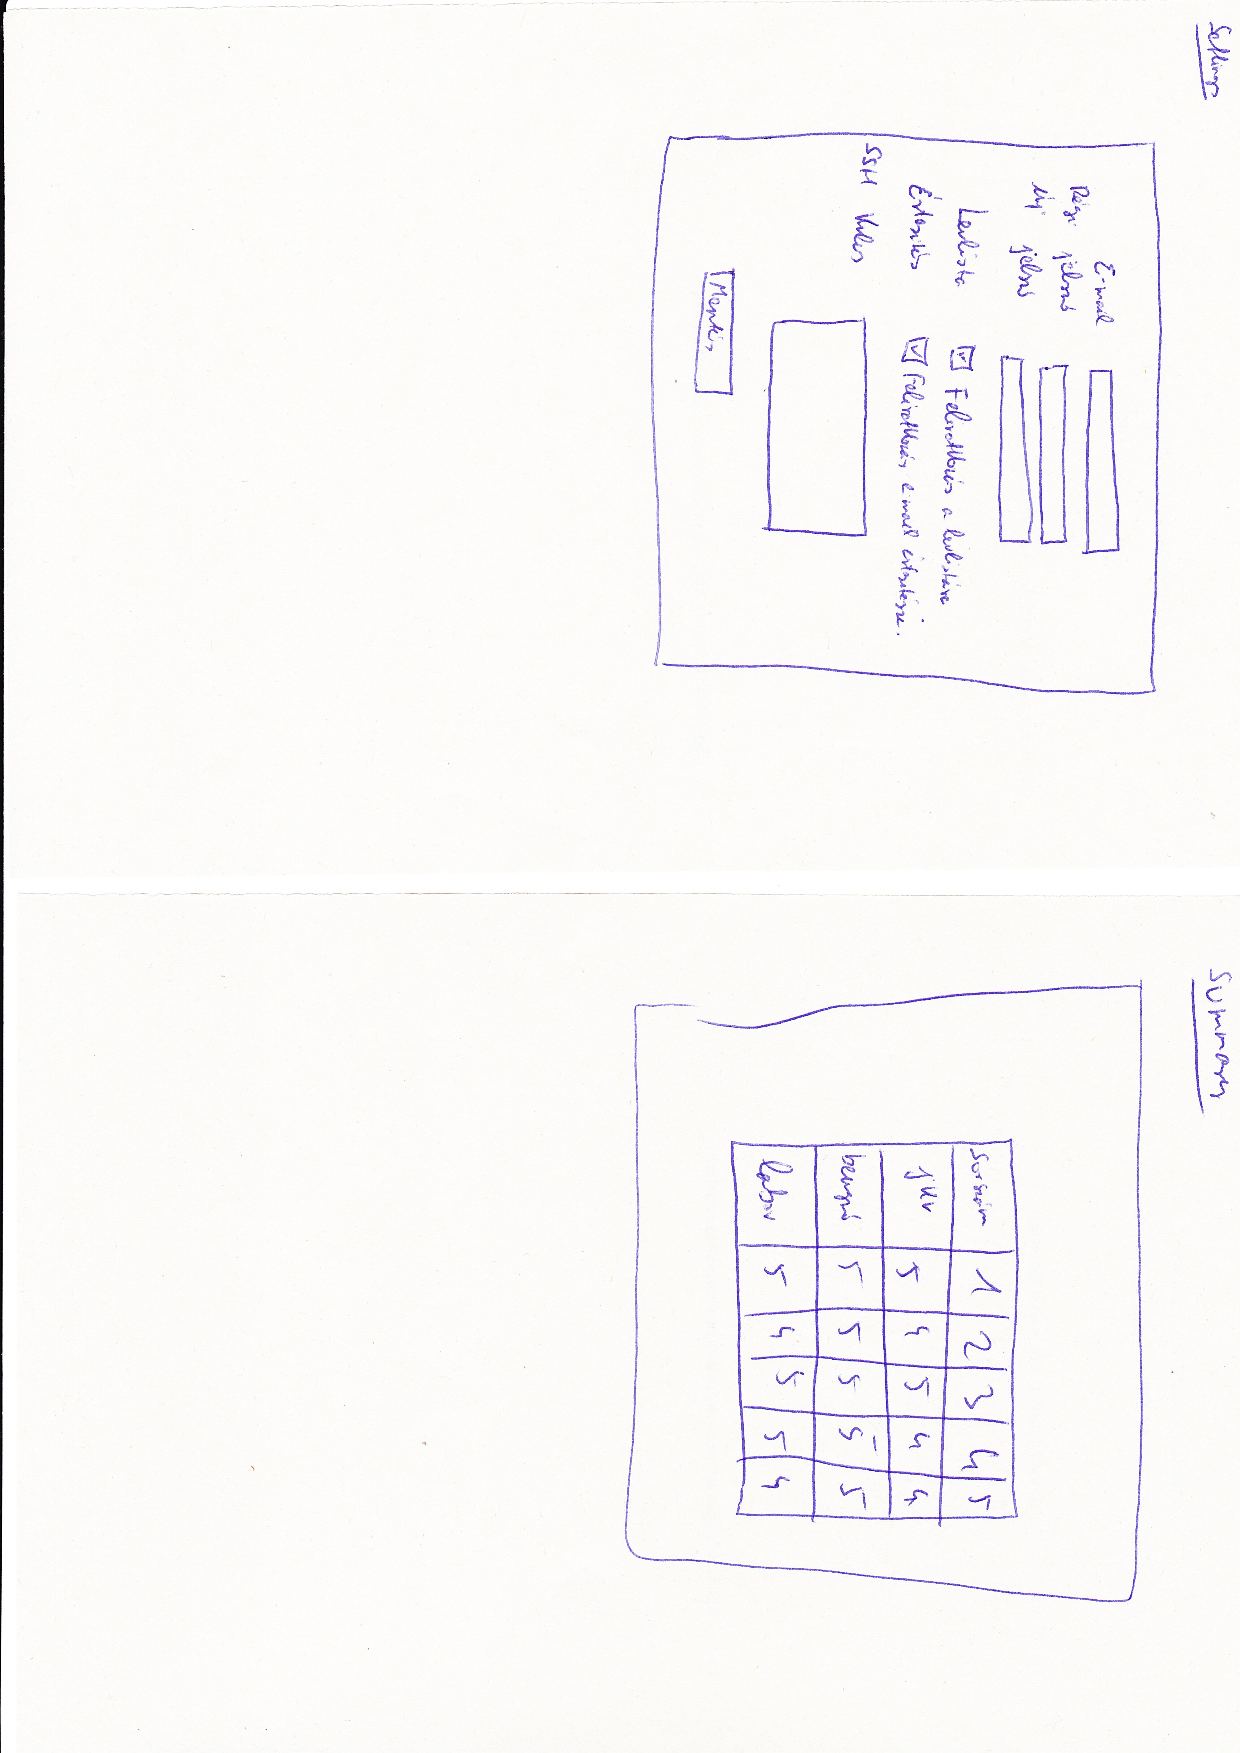
\includepdf[pages=-]{figures/sketches.pdf}
\begin{figure}[!ht]
	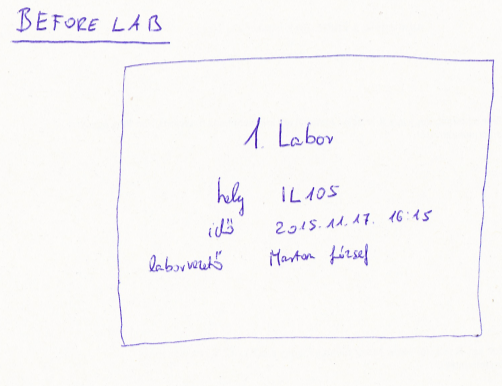
\includegraphics[width=\textwidth]{figures/sketch5.png}
	\caption{Laboratory page sketch, before lab}
	\label{fig:sketch5}
\end{figure}

\begin{figure}[!ht]
	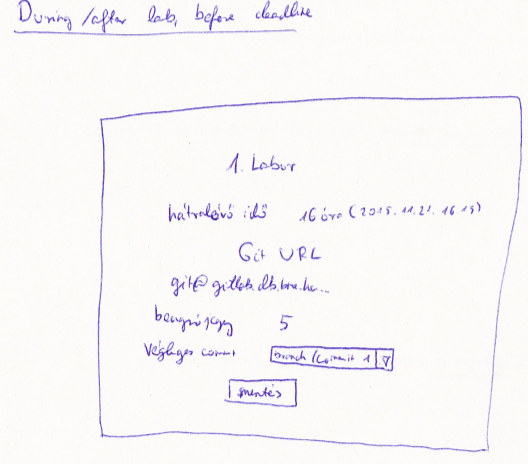
\includegraphics[width=\textwidth]{figures/sketch3.png}
	\caption{Laboratory page sketch, during/after lab, before deadline}
	\label{fig:sketch3}
\end{figure}

\begin{figure}[!ht]
	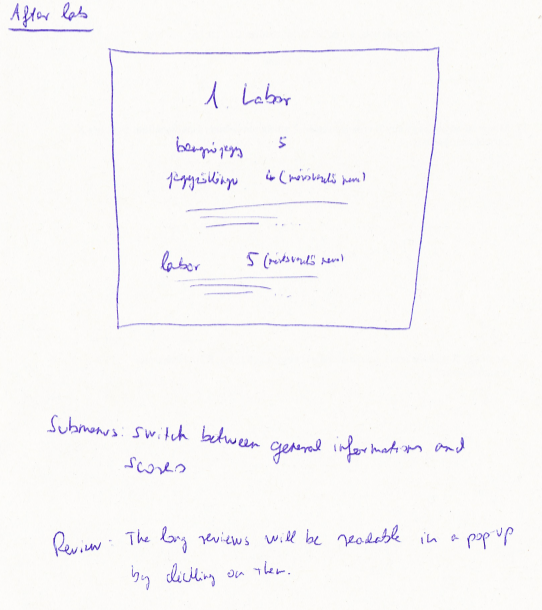
\includegraphics[width=\textwidth]{figures/sketch4.png}
	\caption{Laboratory page sketch, after lab}
	\label{fig:sketch4}
\end{figure}

\begin{figure}[!ht]
	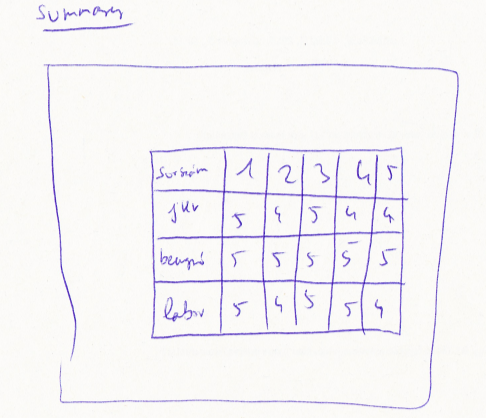
\includegraphics[width=\textwidth]{figures/sketch2.png}
	\caption{Summary page sketch}
	\label{fig:sketch2}
\end{figure}

\begin{figure}[!ht]
	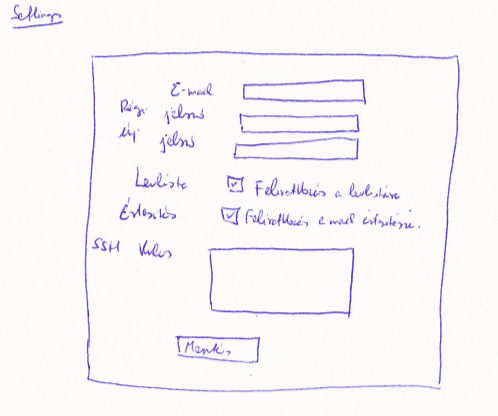
\includegraphics[width=\textwidth]{figures/sketch1.png}
	\caption{Settings page sketch}
	\label{fig:sketch1}
\end{figure}
\chapter{Attribute List}
\label{attribute-list}
\begin{itemize}
	\item Appointments
	\begin{itemize}
		\item attributes
		\begin{itemize}
			\item id - number
			\item date - datetime
			\item location - text
		\end{itemize}
		\item foreign keys
		\begin{itemize}
			\item eventtype - EventTypes
			\item studentgroup - StudentGroups
		\end{itemize}
	\end{itemize}
	
	\item Courses
	\begin{itemize}
		\item attributes
		\begin{itemize}
			\item id - number
			\item name - text
			\item codename - text
		\end{itemize}
	\end{itemize}
	
	\item Deliverables
	\begin{itemize}
		\item attributes
		\begin{itemize}
			\item id - number
			\item deadline - datetime
			\item submitteddate - datetime
			\item grade - number - 1-5
		\end{itemize}
		\item foreign keys
		\begin{itemize}
			\item deliverabletype - DeliverableTypes
			\item evaluator - Staffs
			\item related - Deliverables
		\end{itemize}
		\item Deliverables/Repositories
		\begin{itemize}
			\item attributes
			\begin{itemize}
				\item url - text - type (svn, git) depends on the url
				\item commit - text - chosen final commit
			\end{itemize}
		\end{itemize}
		\item Deliverables/Files
		\begin{itemize}
			\item attributes
			\begin{itemize}
				\item size - number
				\item sha256sum - text
				\item filename - text
			\end{itemize}
		\end{itemize}
	\end{itemize}
	
	\item DeliverableTypes
	\begin{itemize}
		\item attributes
		\begin{itemize}
			\item id - number
			\item type - text - file / repository
			\item deadline - datetime operator - +4 days from the event's date (oracle interval)
			\item description - text - for example: report
		\end{itemize}
		\item foreign keys
		\begin{itemize}
			\item eventtype - EventTypes
		\end{itemize}
	\end{itemize}
	
	\item RegisteredStaffs
	\begin{itemize}
		\item foreign keys
		\begin{itemize}
			\item evaluator - Staffs
			\item exercisetype - ExcerciseTypes
		\end{itemize}
	\end{itemize}
	
	\item Events
	\begin{itemize}
		\item attributes
		\begin{itemize}
			\item id - number
			\item date - datetime
			\item location - text
			\item number - number - 1-5
			\item title - text - DBMS, SQL, JDBC, X*, SOA
			\item attempt - number - starting number: 1
			\item shortdescription - text - generated
		\end{itemize}
		\item foreign keys
		\begin{itemize}
			\item related - Events
			\item eventtype - EventTypes
			\item exercisetype - ExerciseTypes
			\item demonstrator - Staffs
			\item student - Students
			\item studentgroup - StudentGroups			
		\end{itemize}
	\end{itemize}
	
	\item EventTypes
	\begin{itemize}
		\item attributes
		\begin{itemize}
			\item id - number
			\item title - text
			\item number - number
		\end{itemize}
	\end{itemize}
	
	\item ExerciseCategories
	\begin{itemize}
		\item attributes
		\begin{itemize}
			\item id - number
			\item type - text - SQL, DBMS, SOA, JDBC, XML
		\end{itemize}
		\item foreign keys
		\begin{itemize}
			\item course - Courses
		\end{itemize}
	\end{itemize}
	
	\item ExerciseTypes
	\begin{itemize}
		\item attributes
		\begin{itemize}
			\item id - number
			\item name - text - for example: Car Rental
			\item shortname - text - for example: AUTO
			\item exerciseid - number - for example: 22
			\item codename - text - generated, for example: 22-AUTO
			\item language - text
		\end{itemize}
		\item foreign keys
		\begin{itemize}
			\item exercisecategory - ExerciseCategories
		\end{itemize}
	\end{itemize}
	
	\item RegisteredStaffs
	\begin{itemize}
		\item attributes
		\begin{itemize}
			\item id - number
			\item isadmin - boolean
			\item isdemonstrator - boolean
		\end{itemize}
		\item foreign keys
		\begin{itemize}
			\item staff - Staffs
			\item semester - Semesters
		\end{itemize}
	\end{itemize}
	
	\item RegisteredStudents
	\begin{itemize}
		\item attributes
		\begin{itemize}
			\item id - number
			\item neptunsubjectcode - text
			\item neptuncoursecode - text
		\end{itemize}
		\item foreign keys
		\begin{itemize}
			\item student - Students
			\item semester - Semesters
		\end{itemize}
	\end{itemize}
	
	\item Semesters
	\begin{itemize}
		\item attributes
		\begin{itemize}
			\item id - number
			\item academicyear - number
			\item academicterm - number
			\item description - text - generated
		\end{itemize}
		\item foreign keys
		\begin{itemize}
			\item course - Courses
		\end{itemize}
	\end{itemize}
	
	\item StudentGroups
	\begin{itemize}
		\item attributes
		\begin{itemize}
			\item id - number
			\item name - text
			\item language - text
		\end{itemize}
		\item foreign keys
		\begin{itemize}
			\item demonstrator - Staffs
			\item semester - Semesters
		\end{itemize}
	\end{itemize}
	
	\item Users
	\begin{itemize}
		\item attributes
		\begin{itemize}
			\item id - number
			\item givenname - text
			\item surname - text
			\item title - text
			\item displayname - text - generated
			\item loginname - text, unique
			\item eppn - text - Sibboleth
			\item email - text, unique
			\item sshpubliykey - text
			\item password - text
		\end{itemize}
		\item Users/Students
		\begin{itemize}
			\item attributes
			\begin{itemize}
				\item neptun - text
				\item university - text
			\end{itemize}
		\end{itemize}
		\item Users/Staff
	\end{itemize}
\end{itemize}



%\end{appendices}

\label{page:last}
\end{document}
